\documentclass[12pt]{article}

% --- Paquetes (los mismos del template de la tarea) ---
\usepackage{amsmath,amsfonts,amssymb}
\usepackage{enumitem}
\usepackage{graphicx}
\usepackage{fullpage}
\usepackage{algorithm}
\usepackage{algpseudocode}
\usepackage[hidelinks]{hyperref}

% --- Paquetes adicionales que usa el Problema 2 ---
\usepackage[spanish,es-tabla,es-noshorthands]{babel}
\usepackage{booktabs}
\usepackage{float}

% --- Portada ---
\title{\textbf{Análisis y Diseño de Algoritmos Avanzados}\\[0.2cm]\large Capítulo 5 --- Problema 2: Tienda inteligente (Smart Retail Store)}
\author{\small Desiderio Iván Ortegón Mortón, Fernando Robles Vidrio\\[0.1cm]
        \small TC2038 Análisis y Diseño de Algoritmos Avanzados, Gpo.~603, Equipo~8\\
        \small Tecnológico de Monterrey, Campus Monterrey}
\date{\small 9 de noviembre de 2026}

\hypersetup{pdftitle={Assignment 5 - Problema 2: Tienda inteligente (Smart Retail Store)},
            pdfauthor={Desiderio Iván Ortegón Mortón, Fernando Robles Vidrio}}

\begin{document}
\maketitle

% =============================================================================
% Problema 2 -- Smart Retail Store (Assignment 5)
%
% Uso:   % =============================================================================
% Problema 2 -- Smart Retail Store (Assignment 5)
%
% Uso:   % =============================================================================
% Problema 2 -- Smart Retail Store (Assignment 5)
%
% Uso:   \input{problema2} (desde reporte/P2_tienda.tex)
% Paquetes necesarios ademas de los del template: booktabs, float
% Las figuras se leen de figuras/ y las etiquetas usan el prefijo "p2:".
% =============================================================================

\begingroup
\renewcommand{\figurename}{Figura}
\renewcommand{\tablename}{Tabla}
\floatname{algorithm}{Algoritmo}
\algrenewcommand\algorithmicrequire{\textbf{Entrada:}}
\algrenewcommand\algorithmicensure{\textbf{Salida:}}
\algrenewcommand\algorithmicend{\textbf{fin}}
\algrenewcommand\algorithmicwhile{\textbf{mientras}}
\algrenewcommand\algorithmicdo{\textbf{hacer}}
\algrenewcommand\algorithmicif{\textbf{si}}
\algrenewcommand\algorithmicthen{\textbf{entonces}}
\algrenewcommand\algorithmicfor{\textbf{para}}
\algrenewcommand\algorithmicreturn{\textbf{devolver}}
\sloppy

% =============================================================================
\begin{abstract}
\noindent
Una tienda fija precios y coloca guardias, mientras que los clientes \emph{aprenden} si les conviene comprar, robar o irse sin conocer la probabilidad $p$ de ser atrapados (con una multa $f$ si los atrapan). Se ajustó un modelo logístico de compra con descenso de gradiente, demostrando que la pérdida es convexa, y se encontraron tres segmentos de clientes con EM; se optimizó el ingreso no convexo de $d=10$ productos relacionados con gradiente con reinicios, Hill Climbing, Recocido Simulado, un GA real y PSO con el mismo presupuesto de evaluaciones; se colocaron guardias como un juego de Stackelberg resuelto como mochila 0/1 con Branch \& Bound (óptimo de 13 en el caso del enunciado) y se comparó con ACO para 30--120 zonas; se jugó guardia contra ladrón con minimax, alfa-beta y MCTS; y se modeló a los clientes como bandits y como agentes de Q-learning, entrenando la política del guardia con PPO. Los experimentos usan datos de Kaggle (Online Retail II y Retail Price Optimization) y 10 semillas. El B\&B resolvió de forma exacta hasta 120 zonas en menos de 4 ms, el GA fue el método más robusto para los precios, y tanto la cobertura de Stackelberg como la política aprendida con PPO bajaron el robo a $\approx$3\,\%, contra 88\,\% con un guardia predecible.
\end{abstract}

% -----------------------------------------------------------------------------
\section*{Datos y configuración experimental}
\label{p2:sec:datos}

Se usaron dos de los datasets sugeridos, descargados de Kaggle el 9 de noviembre de 2026:
\begin{itemize}[itemsep=1pt]
  \item \textbf{Online Retail II UCI}:\newline \url{https://www.kaggle.com/datasets/mashlyn/online-retail-ii-uci}\newline Archivo \texttt{online\_retail\_II.csv}, con 1\,067\,371 renglones. Se quitaron las filas sin cliente, las facturas canceladas (las que empiezan con ``C''), las cantidades o precios $\le 0$ y los precios mayores al percentil 99.9. Quedaron 804\,774 transacciones de 5\,852 clientes. De aquí salen el modelo de compra, los segmentos de gasto y los valores de los artículos para el problema de los guardias.
  \item \textbf{Retail Price Optimization}:\newline \url{https://www.kaggle.com/datasets/suddharshan/retail-price-optimization}\newline Archivo \texttt{retail\_price.csv}, con 676 renglones. Se agrupó por producto: precio de referencia (mediana de \texttt{unit\_price}), demanda base (media de \texttt{qty}), precio del competidor (mediana de \texttt{comp\_1}) y categoría. De aquí sale el modelo de demanda para los precios.
\end{itemize}
El robo es simulado, con valores de artículos tomados de estos datos, como indica el enunciado.

\begin{table}[H]\centering\small
\begin{tabular}{lp{0.72\linewidth}}\toprule
Equipo & MacBook Pro, Apple M5 Pro, 24 GB de memoria, macOS 26.6.2 \\
Software & Python 3.13.15, NumPy 2.5.4, pandas 3.1.1, scikit-learn 1.9.1, PyTorch 2.15.0, Stable-Baselines3 2.9.2, Gymnasium 1.4.0 \\
Semillas & 10 semillas en todo lo estocástico; se reporta media $\pm$ desviación estándar \\
Tiempo & \texttt{time.perf\_counter} \\
Memoria & pico de \texttt{tracemalloc} en una corrida aparte con la semilla 0 (porque \texttt{tracemalloc} hace más lento el código); para PPO, memoria máxima del proceso \\
Tiempo total & 160 s para todo el problema (40, 43, 28, 5 y 45 s por parte) \\\bottomrule
\end{tabular}
\caption{Configuración de las pruebas.}
\label{p2:tab:setup}
\end{table}

% -----------------------------------------------------------------------------
\section*{1. Modelo de compra (regresión logística) y segmentos de clientes (EM)}
\label{p2:sec:p1}

\paragraph{Modelo de compra.} Para cada cliente se predice si vuelve a comprar en los últimos 90 días del periodo ($y=1$) a partir de su historial anterior a ese corte. Las variables son recencia, frecuencia (número de facturas), monto total, ticket promedio y antigüedad, con $\log(1+x)$ y estandarizadas. Quedaron 5\,256 clientes con historial antes del corte; el 43.6\,\% volvió a comprar.

La pérdida con regularización $\lambda=10^{-3}$ (sin regularizar el sesgo) es
\[ L(\mathbf w) = -\frac1n\sum_{i=1}^n\Big[y_i\log\sigma(\mathbf x_i^\top\mathbf w)+(1-y_i)\log\big(1-\sigma(\mathbf x_i^\top\mathbf w)\big)\Big] + \frac{\lambda}{2}\|\mathbf w_{1:}\|^2, \qquad \sigma(z)=\frac{1}{1+e^{-z}}, \]
y se minimiza con descenso de gradiente, $\mathbf w\gets\mathbf w-\eta\nabla L$, con $\eta=1$, hasta que $\|\nabla L\|<10^{-5}$.

\paragraph{La pérdida es convexa.} Usando $\sigma'(z)=\sigma(z)(1-\sigma(z))$, el gradiente y la Hessiana son
\[ \nabla L = \frac1n X^\top(\boldsymbol\sigma-\mathbf y)+\lambda\,\mathbf w_{1:}, \qquad
   \nabla^2 L = \frac1n X^\top S X + \lambda I', \quad S=\mathrm{diag}\big(\sigma_i(1-\sigma_i)\big), \]
donde $I'$ es la identidad con un cero en la posición del sesgo. Para cualquier vector $\mathbf z$,
\[ \mathbf z^\top\nabla^2 L\,\mathbf z = \frac1n\sum_{i=1}^n \sigma_i(1-\sigma_i)\,(\mathbf x_i^\top\mathbf z)^2 + \lambda\|\mathbf z_{1:}\|^2 \;\ge\; 0, \]
porque $0<\sigma_i<1$. La Hessiana es semidefinida positiva en todo punto, así que $L$ es convexa y cualquier mínimo local es global. Se comprobó también numéricamente: el menor eigenvalor de la Hessiana en la solución es $1.4\times10^{-3}>0$, y al arrancar desde 10 puntos al azar el descenso de gradiente llega siempre a la misma pérdida (0.543046 en los 10 casos, igual hasta la sexta cifra).

\paragraph{Resultados.} Con 10 particiones al azar 80/20, la exactitud en prueba es $0.725\pm0.011$ (adivinar siempre la clase mayoritaria da 0.564) y el AUC es $0.791\pm0.015$. El descenso de gradiente tarda unas 2\,500 iteraciones (0.34 s); son bastantes porque frecuencia, monto y ticket están muy correlacionados. Los pesos tienen el signo esperado: más frecuencia y más monto aumentan la probabilidad de volver, y más días sin comprar la reducen.

\paragraph{Segmentos con EM.} Se ajustó una mezcla de $K$ Gaussianas al logaritmo del gasto total de cada cliente con el algoritmo EM: el paso E calcula la probabilidad de que cada cliente pertenezca a cada componente y el paso M recalcula pesos, medias y varianzas. Se probó $K=1,\dots,5$ con 10 inicializaciones cada uno, y el BIC eligió $K=3$ (Figura~\ref{p2:fig:p1}b):
\begin{itemize}[itemsep=1pt]
  \item segmento 1 (15\,\%): gasto típico de \pounds247, clientes ocasionales;
  \item segmento 2 (71\,\%): gasto típico de \pounds1\,146, la mayoría de los clientes;
  \item segmento 3 (13\,\%): gasto típico de \pounds1\,306 pero con varianza muy grande, porque mezcla clientes pequeños con mayoristas.
\end{itemize}
A diferencia de la logística, EM no es convexo: con $K=3$ la log-verosimilitud final cambia con la semilla (entre $-10\,173.2$ y $-10\,171.3$), porque cada inicialización puede acabar en un máximo local distinto. Por eso se corre con varias semillas y se elige la mejor. El segmento 1 se usa en la parte 2 como los clientes que comparan precios.

\begin{figure}[H]\centering
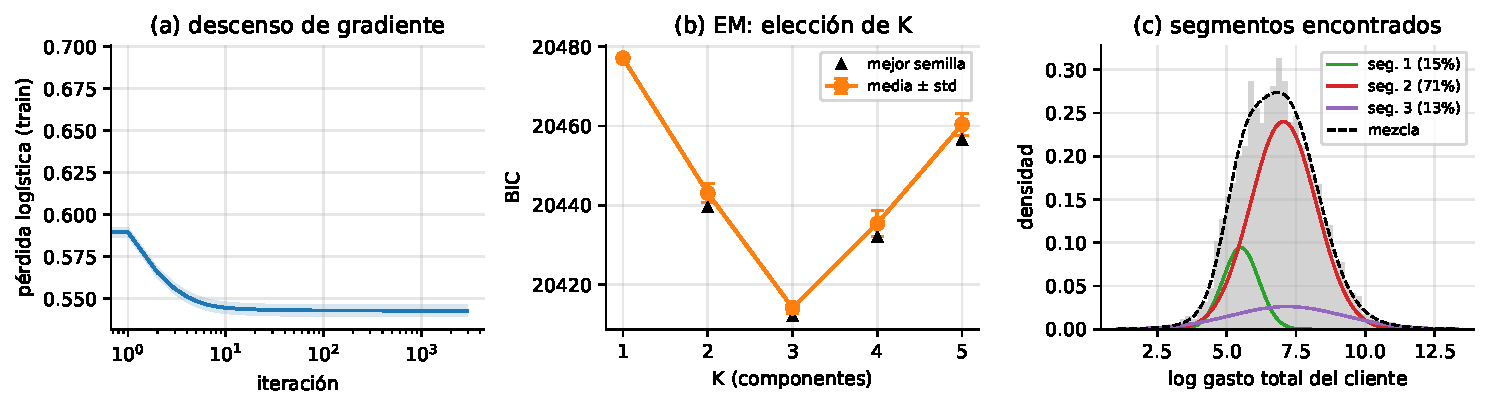
\includegraphics[width=\linewidth]{figuras/p1_logistica_em.pdf}
\caption{(a) Pérdida del descenso de gradiente (10 particiones). (b) BIC contra número de componentes. (c) Mezcla de 3 Gaussianas encontrada por EM sobre el log del gasto.}
\label{p2:fig:p1}
\end{figure}

\paragraph{Escalamiento.} Al pasar de 1\,000 a 5\,852 clientes (5\,256 en la logística, que solo usa clientes con historial antes del corte), el tiempo del descenso de gradiente sube de 0.12 a 0.41 s y el de EM de 0.04 a 0.29 s; la memoria pico, de 0.10 a 0.28 MB y de 0.15 a 0.71 MB (Figura~\ref{p2:fig:p1esc}). Ambos crecen de forma lineal con $n$, como se espera: cada iteración cuesta $O(nd)$ en la logística y $O(nK)$ en EM, y el número de iteraciones casi no cambia.

\begin{figure}[H]\centering
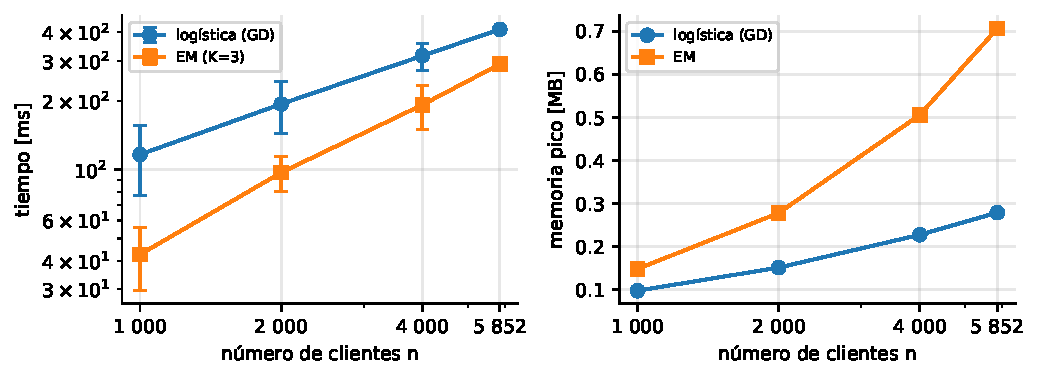
\includegraphics[width=0.8\linewidth]{figuras/p1_escalamiento.pdf}
\caption{Tiempo y memoria pico contra el número de clientes (10 submuestras por tamaño).}
\label{p2:fig:p1esc}
\end{figure}

% -----------------------------------------------------------------------------
\section*{2. Precios de productos relacionados (ingreso no convexo)}
\label{p2:sec:p2}

\paragraph{Modelo.} Se toman los 10 productos con más ventas. Sea $x_i\in[0.5,\,2.5]$ el precio del producto $i$ dividido entre su precio de referencia; la demanda del producto $i$ es
\[ D_i(\mathbf x)= q_i\,e^{-e\,(x_i-1)}\Big[(1-\lambda)+\lambda\,\sigma\big(k\,(c_i-x_i)\big)\Big]\prod_{j\in\text{cat}(i),\,j\ne i}\Big(\frac{x_j}{x_i}\Big)^{g}, \]
y el ingreso es $R(\mathbf x)=\sum_i \text{precio de referencia}_i\, x_i\, D_i(\mathbf x)$. Cada término viene de los datos o de la parte 1:
\begin{itemize}[itemsep=1pt]
  \item $q_i$ es la demanda media del producto y $c_i$ el precio del competidor (\texttt{comp\_1}) relativo al propio.
  \item $\lambda=0.153$ es la fracción de clientes que comparan precios: el peso del segmento de bajo gasto que encontró EM. Si el precio pasa al del competidor, esos clientes se van (la sigmoide $\sigma$).
  \item El último factor relaciona productos de la misma categoría: si uno sube de precio, parte de su demanda pasa a los otros.
  \item Se usaron $e=0.6$, $k=12$ y $g=0.3$.
\end{itemize}

\paragraph{Por qué no es convexo.} Para cada producto hay dos estrategias buenas: quedarse justo debajo del competidor para atraer a los que comparan, o subir mucho el precio y venderle solo a los leales. La Figura~\ref{p2:fig:corte} muestra el ingreso al mover el precio de un solo producto: tiene dos máximos. Con 10 productos las combinaciones se multiplican; al hacer ascenso de gradiente desde 100 puntos al azar se encontraron \textbf{16 óptimos locales distintos}, con ingresos entre 26\,810 y 27\,358.

\begin{figure}[H]\centering
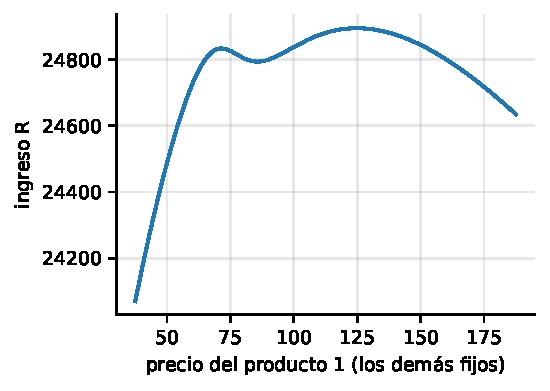
\includegraphics[width=0.42\linewidth]{figuras/p2_corte.pdf}
\caption{Ingreso al variar el precio del producto 1 con los demás fijos: dos máximos locales.}
\label{p2:fig:corte}
\end{figure}

\paragraph{Métodos.} Todos tienen el mismo presupuesto de $300d$ evaluaciones de $R$ (3\,000 para $d=10$):
\begin{itemize}[itemsep=1pt]
  \item \textbf{Gradiente con reinicios}: gradiente por diferencias centrales (cuesta $2d$ evaluaciones), paso de 0.05 en la dirección del gradiente; cuando deja de mejorar, reinicia en un punto al azar.
  \item \textbf{Hill Climbing}: cambia una coordenada con ruido Gaussiano ($\sigma=0.1$) y acepta solo si mejora; reinicia tras 100 intentos sin mejora.
  \item \textbf{Recocido simulado}: como el anterior, pero acepta empeorar con probabilidad $e^{\Delta/T}$; $T$ baja geométricamente durante todo el presupuesto.
  \item \textbf{GA real}: 40 individuos, torneo de 3, cruce BLX-0.5, mutación Gaussiana con probabilidad $1/d$ por gen y elitismo de 2.
  \item \textbf{PSO}: 30 partículas, $w=0.72$, $c_1=c_2=1.49$.
\end{itemize}
Como no se conoce el óptimo global, la brecha se mide contra el mejor ingreso que encontró cualquier método en cualquier semilla.

\begin{table}[H]\centering\footnotesize\setlength{\tabcolsep}{4pt}
\begin{tabular}{lccccc}\toprule
 & \multicolumn{3}{c}{brecha contra el mejor [\%]} & \multicolumn{2}{c}{tiempo [ms]}\\\cmidrule(lr){2-4}\cmidrule(lr){5-6}
Método & $d=10$ & $d=20$ & $d=40$ & $d=10$ & $d=40$\\\midrule
Gradiente + reinicios & 1.00 $\pm$ 0.56 & 21.76 $\pm$ 3.44 & 54.23 $\pm$ 3.24 & 33 & 179 \\
Hill Climbing & 0.43 $\pm$ 0.31 & 0.47 $\pm$ 0.43 & 9.97 $\pm$ 3.52 & 40 & 211 \\
Recocido simulado & 0.55 $\pm$ 0.59 & 0.22 $\pm$ 0.34 & 15.84 $\pm$ 14.07 & 40 & 216 \\
GA real & 0.03 $\pm$ 0.08 & 0.55 $\pm$ 0.37 & 2.15 $\pm$ 2.29 & 92 & 421 \\
PSO & 0.35 $\pm$ 0.40 & 6.16 $\pm$ 3.34 & 20.89 $\pm$ 7.85 & 32 & 180 \\
GA memético (extra) & 0.11 $\pm$ 0.23 & 0.31 $\pm$ 0.32 & 2.67 $\pm$ 2.53 & 75 & 279 \\\bottomrule
\end{tabular}
\caption{Precios: brecha contra el mejor valor encontrado (10 semillas, presupuesto $300d$). Memoria pico: 0.05 MB con $d=10$ y 0.2 MB con $d=40$ en todos los métodos.}
\label{p2:tab:precios}
\end{table}

\paragraph{Resultados.} Con $d=10$ todos los métodos quedan a menos de 1\,\% del mejor; el GA es el más consistente (0.03\,\%). El mejor ingreso encontrado (27\,358) es 10\,\% mayor que el de los precios actuales (24\,826). Al aumentar $d$ las diferencias crecen mucho (Tabla~\ref{p2:tab:precios} y Figura~\ref{p2:fig:p2}):
\begin{itemize}[itemsep=1pt]
  \item El gradiente con reinicios es el peor (54\,\% de brecha con $d=40$): cada gradiente gasta $2d$ evaluaciones, así que con el mismo presupuesto da pocos pasos y queda atrapado en el primer óptimo local.
  \item PSO converge rápido pero se estanca (21\,\% con $d=40$).
  \item Hill Climbing y Recocido Simulado van bien hasta $d=20$, pero con $d=40$ se quedan en 10--16\,\%.
  \item Los dos GA siguen cerca del mejor (2--3\,\%), porque la población explora varias zonas a la vez.
\end{itemize}
El GA es el más lento por el manejo de la población (0.4 s con $d=40$), pero todos son rápidos porque cada evaluación cuesta $O(d^2)$. La memoria crece de forma lineal con $d$ y es igual para todos.

\begin{figure}[H]\centering
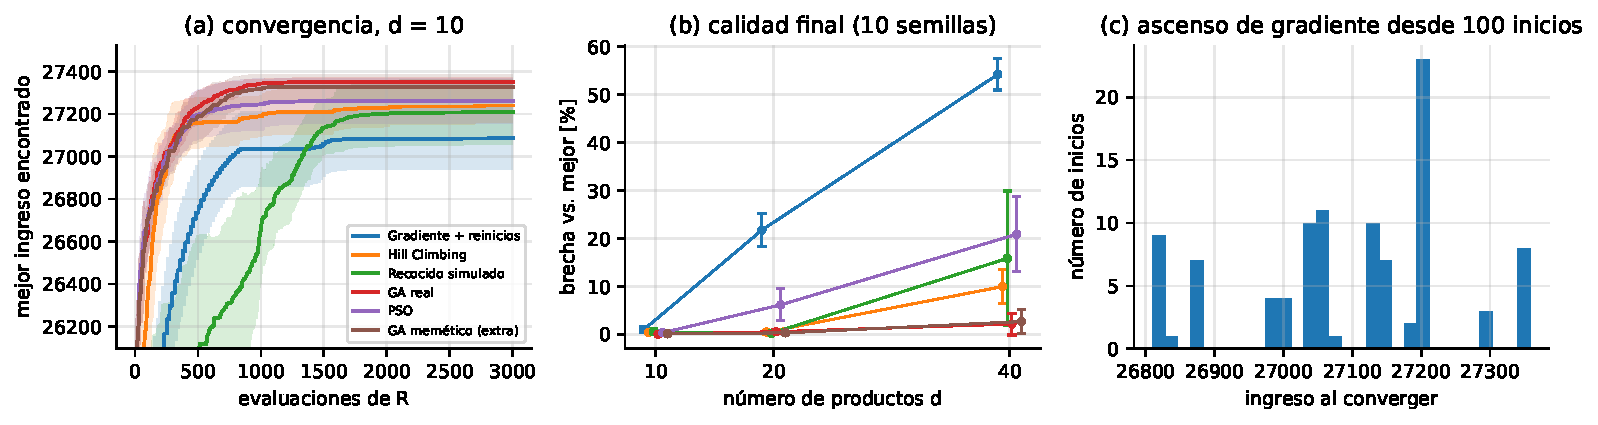
\includegraphics[width=\linewidth]{figuras/p2_precios.pdf}
\caption{(a) Mejor ingreso contra evaluaciones ($d=10$, media $\pm$ desviación). (b) Brecha final contra $d$. (c) Ingreso al que llega el ascenso de gradiente desde 100 inicios distintos.}
\label{p2:fig:p2}
\end{figure}

\begin{figure}[H]\centering
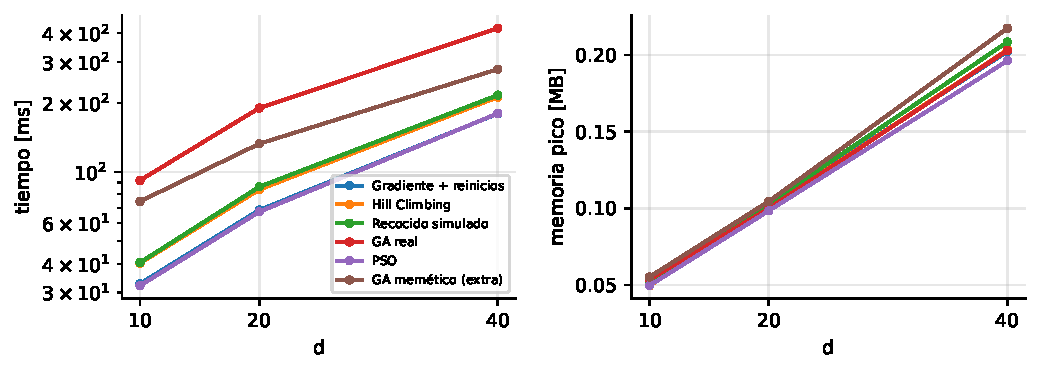
\includegraphics[width=0.8\linewidth]{figuras/p2_escalamiento.pdf}
\caption{Tiempo y memoria pico contra el número de productos.}
\label{p2:fig:p2esc}
\end{figure}

% -----------------------------------------------------------------------------
\section*{3. Guardias como juego de Stackelberg (Branch \& Bound y ACO)}
\label{p2:sec:p3}

\paragraph{Planteamiento.} La tienda (el líder) decide con qué probabilidad $p_z$ vigila cada zona y el ladrón (el seguidor) responde. Si roba en la zona $z$ gana $v_z$ y con probabilidad $p_z$ paga la multa $f$; si no roba se queda con lo que gana por la vía legal, $L$. Le conviene robar si $v_z-p_z f>L$, así que la zona queda disuadida si
\[ p_z\;\ge\;\frac{v_z-L}{f}=c_z. \]
Proteger la zona $z$ cuesta $c_z$ de presupuesto y evita perder $v_z$. Con presupuesto $\sum_z p_z\le B$, elegir qué zonas proteger es una mochila 0/1:
\[ \max\ \sum_z v_z y_z \quad\text{s.a.}\quad \sum_z c_z y_z\le B,\quad y_z\in\{0,1\}. \]

\paragraph{Caso del enunciado.} Con $v=(10,6,3)$, $f=20$, $L=1$ y $B=0.6$, los costos son $c=(0.45,\,0.25,\,0.10)$. Proteger las zonas 1 y 2 cuesta 0.70 (no cabe); proteger las zonas 1 y 3 cuesta 0.55 y vale $10+3=13$; las zonas 2 y 3 valen 9. El Branch \& Bound encuentra el óptimo de \textbf{13} (zonas 1 y 3, con $p_1=0.45$ y $p_3=0.10$) expandiendo 11 nodos, y ACO también llega a 13.

\begin{algorithm}[H]
\caption{Branch \& Bound para la mochila de guardias}
\label{p2:alg:bb}
\begin{algorithmic}[1]
\Require valores $v$, costos $c$, presupuesto $B$
\Ensure valor óptimo y zonas elegidas
\State ordenar zonas por $v_z/c_z$ de mayor a menor; mejor $\gets 0$
\State pila $\gets\{(i=0,\ \text{capacidad}=B,\ \text{valor}=0)\}$
\While{la pila no está vacía}
  \State sacar un nodo; actualizar mejor si su valor es mayor
  \If{$i=n$ \textbf{o} cota fraccionaria$(i,\text{capacidad},\text{valor})\le$ mejor} \textbf{podar} \EndIf
  \State meter ``sin la zona $i$'' (y sin sus copias idénticas)
  \If{$c_i\le$ capacidad} meter ``con la zona $i$'' (se explora primero) \EndIf
\EndWhile
\end{algorithmic}
\end{algorithm}

La cota es la mochila fraccionaria con las zonas que faltan (llenar en orden de $v/c$ y tomar una fracción de la última). Es una cota superior válida, así que podar con ella nunca elimina el óptimo; el código se verificó contra fuerza bruta en 300 instancias pequeñas (\texttt{code/pruebas.py}). La regla de copias idénticas evita explorar soluciones simétricas cuando varias zonas tienen el mismo valor. ACO usa 20 hormigas y 100 iteraciones: cada hormiga agrega zonas que todavía caben con probabilidad proporcional a $\tau^{1}\eta^{2}$, con $\eta=v/c$; la feromona se evapora ($\rho=0.1$) y se refuerza en la mejor solución.

\paragraph{De 30 a 120 zonas.} El valor de cada zona es el precio de un artículo de Online Retail II (en libras, la misma escala que $v=(10,6,3)$). Solo se usan artículos con $v>L$, porque los demás nunca conviene robarlos. El presupuesto es el 30\,\% del costo total y hay 10 instancias por tamaño.

\begin{table}[H]\centering\footnotesize\setlength{\tabcolsep}{4pt}
\begin{tabular}{rrrrrrr}\toprule
Zonas & Óptimo & Nodos B\&B (máx.) & B\&B [ms] & Brecha ACO [\%] & ACO exacto & ACO [ms]\\\midrule
30 & 34.17 & 209 (595) & 0.25 & 0.029 $\pm$ 0.090 & 90\% & 185 \\
60 & 67.39 & 280 (616) & 0.52 & 0.003 $\pm$ 0.009 & 90\% & 381 \\
90 & 102.85 & 654 (1435) & 1.47 & 0.015 $\pm$ 0.031 & 70\% & 574 \\
120 & 138.77 & 649 (1337) & 2.13 & 0.005 $\pm$ 0.011 & 80\% & 809 \\\bottomrule
\end{tabular}
\caption{Mochila de guardias: 10 instancias por tamaño. ``ACO exacto'' es el porcentaje de instancias donde ACO encontró el óptimo exacto. La memoria pico es menor a 0.04 MB en ambos métodos.}
\label{p2:tab:mochila}
\end{table}

El B\&B encontró y \emph{demostró} el óptimo en todas las instancias, con menos de 1\,500 nodos y en menos de 4 ms. ACO llega a menos de 0.03\,\% en promedio y encuentra el óptimo exacto en 70--90\,\% de las instancias, pero tarda entre 380 y 740 veces más y no puede garantizar que su solución sea la óptima (Figura~\ref{p2:fig:p3}). Aun así, el B\&B es exponencial en el peor caso: cuando valor y costo son casi proporcionales la cota fraccionaria poda poco. En estos datos no pasó porque la mayoría de los artículos son baratos y la razón $v/c=fv/(v-L)$ varía mucho entre zonas.

\begin{figure}[H]\centering
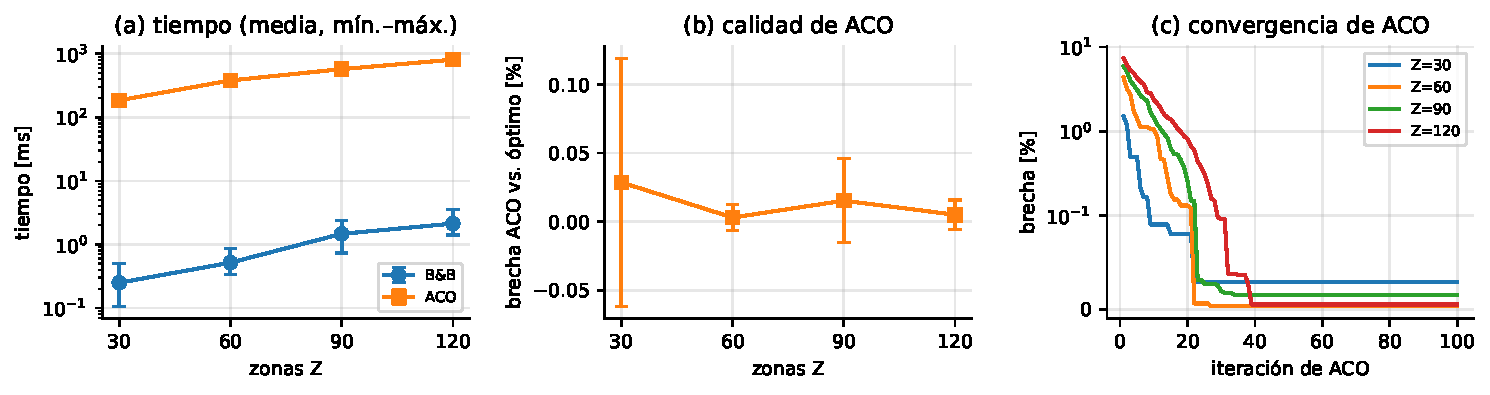
\includegraphics[width=\linewidth]{figuras/p3_mochila.pdf}
\caption{(a) Tiempo de B\&B y ACO. (b) Brecha de ACO contra el óptimo de B\&B. (c) Convergencia de ACO por iteración (promedio de 10 instancias).}
\label{p2:fig:p3}
\end{figure}

% -----------------------------------------------------------------------------
\section*{4. Guardia contra ladrón: minimax, alfa-beta y MCTS}
\label{p2:sec:p4}

\paragraph{Juego.} La tienda es una cuadrícula $n\times n$ con la salida en una esquina y tres zonas con artículos de valor 10, 6 y 3. El ladrón y el guardia se mueven por turnos una casilla (o se quedan). Si el ladrón pisa una zona toma el artículo. Las reglas para terminar son:
\begin{itemize}[itemsep=1pt]
  \item si el guardia llega a la casilla del ladrón, lo atrapa y la utilidad es $-20$ (la multa);
  \item si el ladrón llega a la salida con botín, escapa y la utilidad es el botín;
  \item si se acaban los turnos, la utilidad es 0.
\end{itemize}
Es un juego de suma cero: el ladrón maximiza y el guardia minimiza. Cuando la búsqueda se corta, una función de evaluación estima el valor con el botín (descontado por la distancia a la salida), la cercanía a los artículos que quedan y la cercanía al guardia.

\paragraph{Métodos.}
\begin{itemize}[itemsep=1pt]
  \item \textbf{Minimax} con profundidad limitada.
  \item \textbf{Alfa-beta} con dos órdenes de jugadas: aleatorio, o ``bueno'' (primero las jugadas con mejor evaluación para quien mueve).
  \item \textbf{MCTS con UCT}: 500 iteraciones de selección con $\bar u+1.4\sqrt{\ln N/n}$, expansión, simulación aleatoria hasta el final y retropropagación.
\end{itemize}

\begin{table}[H]\centering\small
\begin{tabular}{llrrr}\toprule
Cuadrícula & Profundidad & Minimax & Alfa-beta (aleatorio) & Alfa-beta (buen orden)\\\midrule
5$\times$5 & 2 & 17 & 13 & 10 \\
5$\times$5 & 4 & 289 & 130 & 70 \\
5$\times$5 & 6 & 4\,864 & 880 & 385 \\
5$\times$5 & 8 & -- & 5\,996 & 1\,771 \\
4$\times$4 & 8 & 63\,874 & 4\,668 & 1\,411 \\
6$\times$6 & 8 & -- & 7\,289 & 1\,395 \\\bottomrule
\end{tabular}
\caption{Nodos expandidos para decidir la primera jugada (promedio de 10 tableros). ``--'': no se corrió minimax a profundidad 8 en tableros grandes por ser demasiado lento.}
\label{p2:tab:nodos}
\end{table}

\paragraph{Resultados de la búsqueda.} En los 120 casos probados (100 con minimax, que no se corrió a profundidad 8 en $5\times5$ ni en $6\times6$), todas las variantes dieron exactamente el mismo valor en la raíz: la poda no cambia el resultado, solo evita trabajo. El ahorro crece con la profundidad (Tabla~\ref{p2:tab:nodos} y Figura~\ref{p2:fig:p4}):
\begin{itemize}[itemsep=1pt]
  \item a profundidad 6, alfa-beta con buen orden expande 12.6 veces menos nodos que minimax;
  \item en $4\times4$ a profundidad 8, el ahorro es de 45 veces (63\,874 contra 1\,411 nodos).
\end{itemize}
El factor de ramificación efectivo ($N^{1/d}$) a profundidad 6 en $5\times5$ es 4.1 con minimax, 3.1 con alfa-beta en orden aleatorio y 2.7 con buen orden, que se acerca al mínimo teórico de $\sqrt{4.1}\approx2.0$. El tamaño del tablero casi no influye, porque cada jugador tiene a lo más 5 movimientos sin importar $n$. La memoria de minimax y alfa-beta es mínima (0.001 MB, solo la pila de recursión); la de MCTS es mayor (0.23 MB) porque guarda el árbol.

\begin{figure}[H]\centering
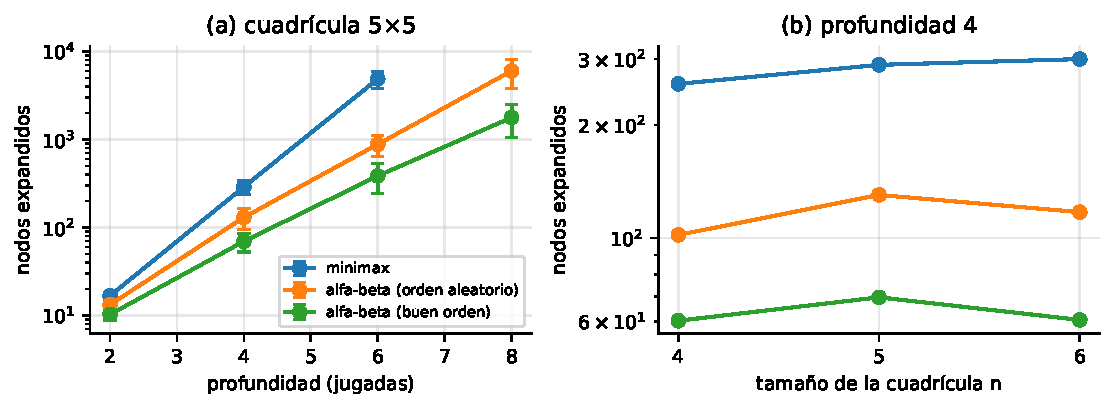
\includegraphics[width=0.8\linewidth]{figuras/p4_busqueda.pdf}
\caption{Nodos expandidos: (a) contra la profundidad en $5\times5$; (b) contra el tamaño del tablero a profundidad 4.}
\label{p2:fig:p4}
\end{figure}

\begin{table}[H]\centering\footnotesize\setlength{\tabcolsep}{4pt}
\begin{tabular}{llrrrrr}\toprule
Ladrón & Guardia & Utilidad ladrón & Escapa & Atrapado & $t$ ladrón [ms] & $t$ guardia [ms]\\\midrule
alfa-beta $p=4$ & alfa-beta $p=4$ & 0.9 $\pm$ 2.0 & 20\% & 0\% & 2 & 2 \\
alfa-beta $p=4$ & MCTS 500 & 2.2 $\pm$ 5.2 & 20\% & 0\% & 2 & 79 \\
MCTS 500 & alfa-beta $p=4$ & 0.3 $\pm$ 0.9 & 10\% & 0\% & 71 & 2 \\
MCTS 500 & MCTS 500 & 1.3 $\pm$ 3.2 & 20\% & 0\% & 73 & 70 \\
alfa-beta $p=4$ & aleatorio & 4.5 $\pm$ 6.6 & 40\% & 0\% & 2 & 0 \\\bottomrule
\end{tabular}
\caption{Partidas completas en $5\times5$ con 24 jugadas como máximo (10 tableros distintos). Los tiempos son el total de decisión por partida.}
\label{p2:tab:partidas}
\end{table}

\paragraph{Partidas.} El guardia con alfa-beta es el que menos deja ganar al ladrón, y uno que se mueve al azar deja escapar al 40\,\% de los ladrones (Tabla~\ref{p2:tab:partidas}). Nunca atrapan al ladrón, porque la multa de $-20$ hace que este prefiera irse sin nada antes que arriesgarse. MCTS juega de forma comparable a alfa-beta sin necesitar función de evaluación, pero tarda unas 35 veces más por partida porque cada iteración simula el juego hasta el final.

% -----------------------------------------------------------------------------
\section*{5. Clientes que aprenden: bandits, Q-learning y PPO}
\label{p2:sec:p5}

\paragraph{Bandits.} Un cliente frente a un artículo de valor $v=10$ con precio 9 tiene tres opciones, sin conocer $p$:
\begin{itemize}[itemsep=1pt]
  \item comprar: gana $v-\text{precio}=L=1$, más ruido $\mathcal N(0,1)$;
  \item robar: gana 10, o $10-20=-10$ si lo atrapan;
  \item irse: gana 0, más ruido.
\end{itemize}
Robar conviene si $10-20p>1$, es decir si $p<p^\star=(v-L)/f=0.45$, el mismo umbral de la parte 3. Se compararon tres estrategias en $2\times10^4$ visitas y 10 semillas:
\begin{itemize}[itemsep=1pt]
  \item $\varepsilon$-greedy con $\varepsilon=0.1$;
  \item UCB1, con las recompensas reescaladas a $[0,1]$;
  \item Thompson sampling con posterior Gaussiana ($\sigma=10$).
\end{itemize}

\begin{table}[H]\centering\footnotesize\setlength{\tabcolsep}{4pt}
\begin{tabular}{rlrrrrr}\toprule
$p$ & Algoritmo & Regret final & Robo (total) & Robo (últ. 1000) & Tiempo [ms] & Memoria [MB]\\\midrule
0.30 & Thompson & 610 $\pm$ 82 & 99.1\% & 99.9\% & 105 & 0.32 \\
0.30 & UCB1 & 4\,439 $\pm$ 212 & 93.4\% & 98.1\% & 81 & 0.31 \\
0.30 & $\varepsilon$-greedy & 5\,076 $\pm$ 654 & 92.7\% & 93.3\% & 38 & 0.31 \\
0.60 & Thompson & 911 $\pm$ 165 & 0.5\% & 0.1\% & 103 & 0.32 \\
0.60 & UCB1 & 5\,695 $\pm$ 474 & 4.0\% & 1.6\% & 83 & 0.31 \\
0.60 & $\varepsilon$-greedy & 2\,755 $\pm$ 110 & 3.4\% & 3.3\% & 40 & 0.31 \\\bottomrule
\end{tabular}
\caption{Bandits con $2\times10^4$ visitas y 10 semillas. Regret $=\sum_t(\mu^\star-\mu_{a_t})$.}
\label{p2:tab:bandits}
\end{table}

Los clientes aprenden lo correcto: con $p=0.30$ terminan robando casi siempre y con $p=0.60$ casi nunca (Tabla~\ref{p2:tab:bandits}). Thompson tiene el menor regret en ambos casos. $\varepsilon$-greedy tiene regret lineal, porque explora el 10\,\% del tiempo para siempre. UCB1 explora mucho al principio, porque las recompensas van de $-10$ a 10 y sus intervalos de confianza son anchos; aun así su regret crece de forma logarítmica. El barrido de $p$ (Figura~\ref{p2:fig:bandits}c) muestra que el cliente pasa de robar a no robar justo alrededor de $p^\star=0.45$: con $p=0.40$ roba el 69\,\% de las veces, con $p=0.45$ el 41\,\% y con $p=0.50$ el 17\,\%.

\begin{figure}[H]\centering
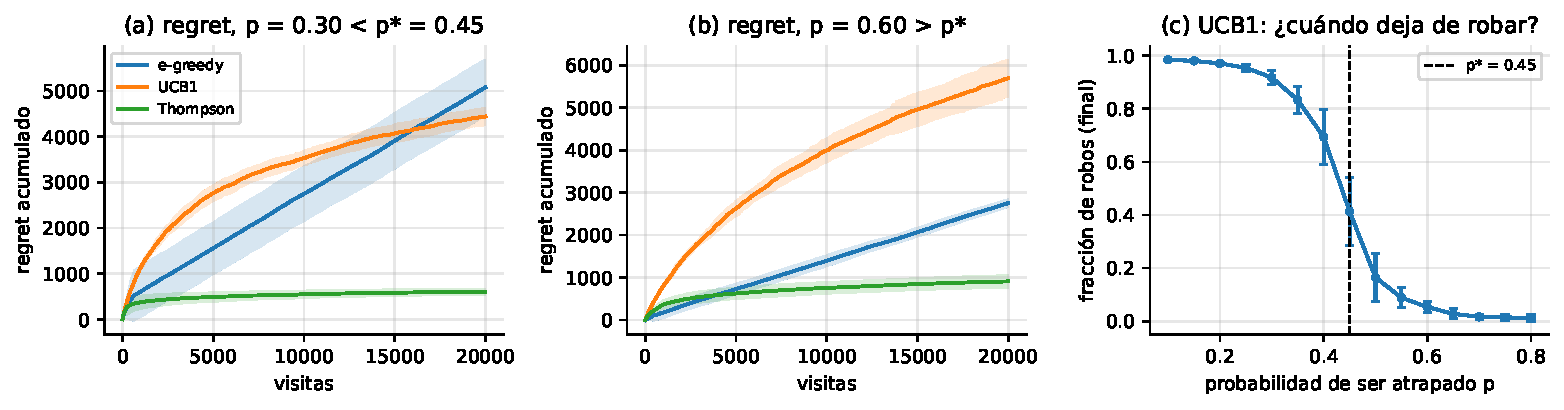
\includegraphics[width=\linewidth]{figuras/p5_bandits.pdf}
\caption{(a, b) Regret acumulado con $p$ debajo y encima de $p^\star$. (c) Fracción de robos al final contra $p$ (UCB1).}
\label{p2:fig:bandits}
\end{figure}

\paragraph{Q-learning con el guardia visible.} La tienda tiene tres zonas ($v=10,6,3$). El cliente ve en qué zona está el guardia al entrar ($g_0$), elige a qué zona ir y luego si compra, roba o se va. Mientras tanto el guardia se mueve a $g_1$ según la política de la tienda. Si roba en la zona donde quedó el guardia lo atrapan con probabilidad 0.9; en las demás, la cámara lo atrapa con probabilidad 0.05. El cliente aprende con Q-learning tabular: estado $g_0$ y luego $(g_0,\text{zona})$, $\varepsilon=0.1$, tasa $\alpha=\max(1/n,\,0.02)$.

Se probaron cuatro políticas fijas de la tienda. La política de Stackelberg usa la cobertura mínima que disuade todas las zonas, $0.9\,c_z+0.05\,(1-c_z)\ge(v_z-L)/f$, repartiendo el resto en proporción: $c=(0.62,\,0.31,\,0.08)$.

\paragraph{PPO para el guardia.} La tienda aprende su política con PPO de Stable-Baselines3 contra clientes que siguen aprendiendo con Q-learning:
\begin{itemize}[itemsep=1pt]
  \item \textbf{Observación:} zona actual del guardia y tasa reciente de robos por zona.
  \item \textbf{Acción:} a qué zona moverse.
  \item \textbf{Recompensa:} menos el valor robado.
  \item \textbf{Entrenamiento:} $2\times10^4$ visitas por semilla, con $\gamma=0$ (cada visita se paga sola), \texttt{n\_steps}=1000, \texttt{batch\_size}=200, 10 épocas, tasa de aprendizaje $10^{-3}$ y coeficiente de entropía 0.02.
\end{itemize}

\begin{table}[H]\centering\small
\begin{tabular}{lrrrr}\toprule
Política del guardia & Robo (todo) & Robo (últimas 2000) & Pérdida por visita & Tiempo [s]\\\midrule
fijo en zona 1 & 87.4 $\pm$ 0.8\% & 88.3 $\pm$ 0.8\% & 4.96 $\pm$ 0.06 & 0.08 \\
rotación 1$\to$2$\to$3 & 86.4 $\pm$ 1.7\% & 88.1 $\pm$ 0.5\% & 7.09 $\pm$ 0.26 & 0.08 \\
uniforme & 59.1 $\pm$ 15.7\% & 60.7 $\pm$ 20.9\% & 4.02 $\pm$ 1.41 & 0.09 \\
Stackelberg (mixta) & 4.9 $\pm$ 0.9\% & 3.4 $\pm$ 1.0\% & 0.11 $\pm$ 0.03 & 0.21 \\
PPO (aprendida) & 10.7 $\pm$ 2.9\% & 3.3 $\pm$ 0.3\% & 0.11 $\pm$ 0.02 & 2.88 \\\bottomrule
\end{tabular}
\caption{Clientes con Q-learning contra distintas políticas del guardia ($2\times10^4$ visitas, 10 semillas).}
\label{p2:tab:guardia}
\end{table}

\paragraph{Resultados.} Las políticas predecibles fallan: si el guardia siempre está en la misma zona o rota en orden fijo, el cliente aprende dónde va a estar y roba en otra zona el 88\,\% de las veces. La uniforme no alcanza, porque la zona 1 necesita al menos 0.47 de cobertura y solo recibe $1/3$. La mezcla de Stackelberg baja el robo a 3.4\,\%. PPO, sin conocer el modelo, llega al mismo nivel (3.3\,$\pm$\,0.3\,\% al final, en las 10 semillas). La cobertura promedio que aprendió, $(0.52,\,0.30,\,0.18)$, cumple los tres umbrales: las probabilidades de atrapar son 0.49, 0.30 y 0.20, contra los mínimos de 0.45, 0.25 y 0.10. El piso de $\approx$3\,\% no se puede bajar con vigilancia: es la exploración de los clientes ($\varepsilon/3\approx0.033$ de robos al azar). El costo de aprender es que durante el entrenamiento el robo promedio es 10.7\,\%, y que PPO tarda 2.9 s por semilla contra 0.2 s de la política calculada; además necesita PyTorch, y la memoria máxima del proceso llegó a 750 MB (esta cifra incluye los datos cargados en las partes anteriores).

\begin{figure}[H]\centering
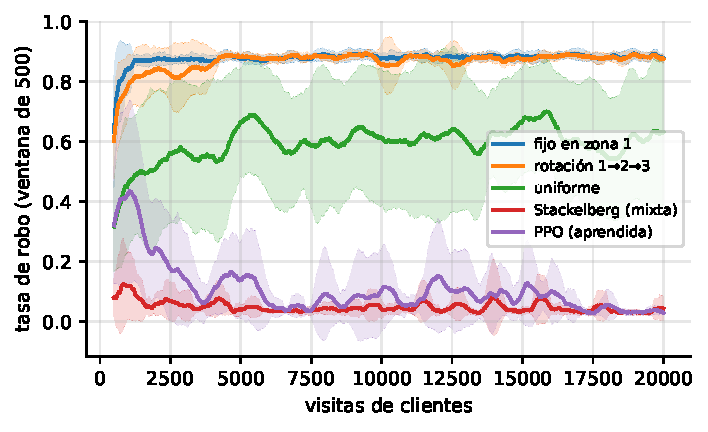
\includegraphics[width=0.72\linewidth]{figuras/p5_guardia.pdf}
\caption{Tasa de robo (ventana de 500 visitas) según la política del guardia; media $\pm$ desviación de 10 semillas.}
\label{p2:fig:guardia}
\end{figure}

% -----------------------------------------------------------------------------
\section*{Discusión: qué fue convexo y cuándo planear o aprender}
\label{p2:sec:discusion}

\paragraph{Convexo y no convexo.}
\begin{itemize}[itemsep=1pt]
  \item \textbf{Convexos:} la pérdida logística (demostrado arriba), por eso el descenso de gradiente llega al mismo mínimo desde cualquier inicio; y la mochila fraccionaria, que es un problema lineal y sirve como cota en el B\&B.
  \item \textbf{No convexos:} la verosimilitud de EM (el resultado depende de la semilla), el ingreso de los productos (16 óptimos locales), la mochila 0/1 (es discreta), los juegos de búsqueda y el objetivo de PPO (una red neuronal contra un rival que cambia).
\end{itemize}
En lo convexo basta un método local; en lo no convexo hacen falta reinicios, poblaciones (GA, PSO, ACO) o búsqueda exacta con cotas.

\paragraph{Planear o aprender.} Conviene \emph{planear} con búsqueda exacta y cotas válidas cuando el modelo se conoce y el problema es chico:
\begin{itemize}[itemsep=1pt]
  \item el B\&B resolvió la mochila de guardias de forma exacta en milisegundos, mientras que ACO tardó cientos de veces más sin garantía;
  \item alfa-beta da la misma jugada que minimax (la óptima para la profundidad elegida) expandiendo muchos menos nodos y con poca memoria.
\end{itemize}
Conviene \emph{aprender} cuando no se conocen los parámetros ($p$, el comportamiento de los clientes) o cuando el rival se adapta. Los bandits encuentran el umbral $p^\star$ sin conocerlo, y PPO recuperó una estrategia equivalente a la de Stackelberg sin saber nada del modelo. A cambio, aprender necesitó miles de interacciones (con robos mientras aprendía), más tiempo y mucha más memoria que calcular la solución. En la práctica, la tienda debería planear con lo que sabe (la cobertura de Stackelberg) y usar el aprendizaje para ajustar cuando los datos reales no coinciden con el modelo.

% -----------------------------------------------------------------------------
\section*{Crédito extra}
\label{p2:sec:extra}

\paragraph{Modelo híbrido búsqueda--bioinspirado (GA memético).} Es el mismo GA real, pero en cada generación se aplica Hill Climbing ($2d$ pasos) al mejor individuo; las evaluaciones del Hill Climbing cuentan dentro del mismo presupuesto. Así, el GA explora y el Hill Climbing refina. Con $d=20$ fue el mejor de los métodos bioinspirados (0.31\,\% contra 0.55\,\% del GA), con $d=40$ quedó prácticamente empatado con el GA (2.7\,\% contra 2.2\,\%, dentro de la desviación estándar), y en los tres tamaños superó a Hill Climbing y a PSO; a Recocido Simulado lo superó con $d=10$ y $d=40$, aunque con $d=20$ Recocido quedó un poco mejor (0.22\,\% contra 0.31\,\%) (Tabla~\ref{p2:tab:precios}).

\paragraph{Tablero de visualización.} El programa genera \texttt{results/dashboard.html}, una página que se abre en el navegador con un panel por parte y las tablas resumen. También genera la Figura~\ref{p2:fig:dashboard}.

\begin{figure}[H]\centering
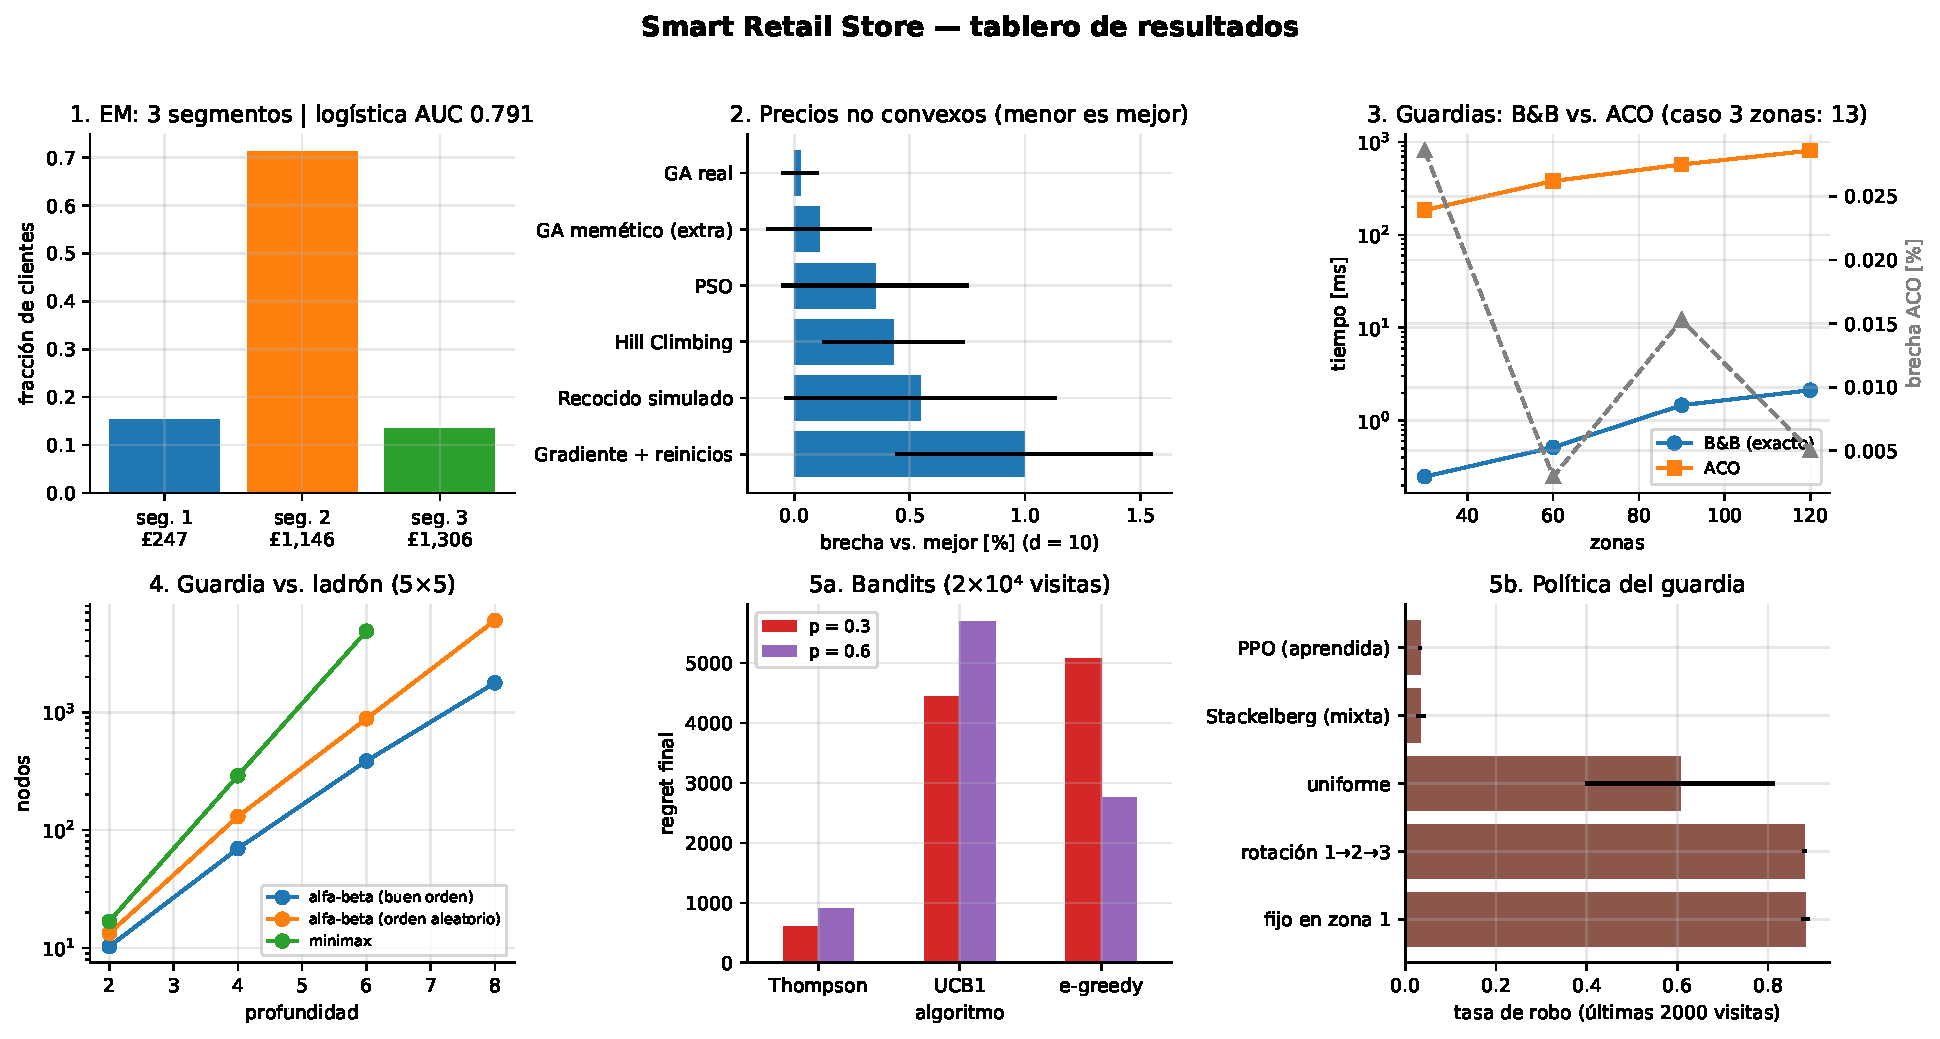
\includegraphics[width=\linewidth]{figuras/dashboard.pdf}
\caption{Tablero de resultados del Problema 2.}
\label{p2:fig:dashboard}
\end{figure}

\paragraph{Reproducir.} Las instrucciones para instalar las dependencias, descargar los datos y correr los experimentos están en el archivo \texttt{README.md} de la carpeta \texttt{problema2} del repositorio.

% -----------------------------------------------------------------------------
\section*{Referencias}
{\raggedright
\begin{enumerate}[label={[\arabic*]},leftmargin=*,itemsep=1pt]
\item S. Russell y P. Norvig. \emph{Artificial Intelligence: A Modern Approach}, 4.\textsuperscript{a} ed. Pearson, 2021.
\item A. P. Dempster, N. M. Laird y D. B. Rubin. Maximum likelihood from incomplete data via the EM algorithm. \emph{Journal of the Royal Statistical Society: Series B} 39(1):1--38, 1977.
\item S. Kirkpatrick, C. D. Gelatt y M. P. Vecchi. Optimization by simulated annealing. \emph{Science} 220(4598):671--680, 1983.
\item L. J. Eshelman y J. D. Schaffer. Real-coded genetic algorithms and interval-schemata. En \emph{Foundations of Genetic Algorithms 2}, pp.~187--202. Morgan Kaufmann, 1993.
\item J. Kennedy y R. Eberhart. Particle swarm optimization. En \emph{Proc. IEEE International Conference on Neural Networks}, pp.~1942--1948, 1995.
\item M. Tambe. \emph{Security and Game Theory: Algorithms, Deployed Systems, Lessons Learned}. Cambridge University Press, 2011.
\item M. Dorigo y T. Stützle. \emph{Ant Colony Optimization}. MIT Press, 2004.
\item D. E. Knuth y R. W. Moore. An analysis of alpha-beta pruning. \emph{Artificial Intelligence} 6(4):293--326, 1975.
\item L. Kocsis y C. Szepesvári. Bandit based Monte-Carlo planning. En \emph{Machine Learning: ECML 2006}, LNCS 4212, pp.~282--293. Springer, 2006.
\item P. Auer, N. Cesa-Bianchi y P. Fischer. Finite-time analysis of the multiarmed bandit problem. \emph{Machine Learning} 47:235--256, 2002.
\item W. R. Thompson. On the likelihood that one unknown probability exceeds another in view of the evidence of two samples. \emph{Biometrika} 25(3/4):285--294, 1933.
\item C. J. C. H. Watkins y P. Dayan. Q-learning. \emph{Machine Learning} 8:279--292, 1992.
\item J. Schulman, F. Wolski, P. Dhariwal, A. Radford y O. Klimov. Proximal policy optimization algorithms. arXiv:1707.06347, 2017.
\item A. Raffin, A. Hill, A. Gleave, A. Kanervisto, M. Ernestus y N. Dormann. Stable-Baselines3: reliable reinforcement learning implementations. \emph{Journal of Machine Learning Research} 22(268):1--8, 2021.
\item Online Retail II UCI (Kaggle). \url{https://www.kaggle.com/datasets/mashlyn/online-retail-ii-uci}, consultado el 9 de noviembre de 2026.
\item Retail Price Optimization (Kaggle). \url{https://www.kaggle.com/datasets/suddharshan/retail-price-optimization}, consultado el 9 de noviembre de 2026.
\end{enumerate}
\par}

\clearpage
\endgroup
 (desde reporte/P2_tienda.tex)
% Paquetes necesarios ademas de los del template: booktabs, float
% Las figuras se leen de figuras/ y las etiquetas usan el prefijo "p2:".
% =============================================================================

\begingroup
\renewcommand{\figurename}{Figura}
\renewcommand{\tablename}{Tabla}
\floatname{algorithm}{Algoritmo}
\algrenewcommand\algorithmicrequire{\textbf{Entrada:}}
\algrenewcommand\algorithmicensure{\textbf{Salida:}}
\algrenewcommand\algorithmicend{\textbf{fin}}
\algrenewcommand\algorithmicwhile{\textbf{mientras}}
\algrenewcommand\algorithmicdo{\textbf{hacer}}
\algrenewcommand\algorithmicif{\textbf{si}}
\algrenewcommand\algorithmicthen{\textbf{entonces}}
\algrenewcommand\algorithmicfor{\textbf{para}}
\algrenewcommand\algorithmicreturn{\textbf{devolver}}
\sloppy

% =============================================================================
\begin{abstract}
\noindent
Una tienda fija precios y coloca guardias, mientras que los clientes \emph{aprenden} si les conviene comprar, robar o irse sin conocer la probabilidad $p$ de ser atrapados (con una multa $f$ si los atrapan). Se ajustó un modelo logístico de compra con descenso de gradiente, demostrando que la pérdida es convexa, y se encontraron tres segmentos de clientes con EM; se optimizó el ingreso no convexo de $d=10$ productos relacionados con gradiente con reinicios, Hill Climbing, Recocido Simulado, un GA real y PSO con el mismo presupuesto de evaluaciones; se colocaron guardias como un juego de Stackelberg resuelto como mochila 0/1 con Branch \& Bound (óptimo de 13 en el caso del enunciado) y se comparó con ACO para 30--120 zonas; se jugó guardia contra ladrón con minimax, alfa-beta y MCTS; y se modeló a los clientes como bandits y como agentes de Q-learning, entrenando la política del guardia con PPO. Los experimentos usan datos de Kaggle (Online Retail II y Retail Price Optimization) y 10 semillas. El B\&B resolvió de forma exacta hasta 120 zonas en menos de 4 ms, el GA fue el método más robusto para los precios, y tanto la cobertura de Stackelberg como la política aprendida con PPO bajaron el robo a $\approx$3\,\%, contra 88\,\% con un guardia predecible.
\end{abstract}

% -----------------------------------------------------------------------------
\section*{Datos y configuración experimental}
\label{p2:sec:datos}

Se usaron dos de los datasets sugeridos, descargados de Kaggle el 9 de noviembre de 2026:
\begin{itemize}[itemsep=1pt]
  \item \textbf{Online Retail II UCI}:\newline \url{https://www.kaggle.com/datasets/mashlyn/online-retail-ii-uci}\newline Archivo \texttt{online\_retail\_II.csv}, con 1\,067\,371 renglones. Se quitaron las filas sin cliente, las facturas canceladas (las que empiezan con ``C''), las cantidades o precios $\le 0$ y los precios mayores al percentil 99.9. Quedaron 804\,774 transacciones de 5\,852 clientes. De aquí salen el modelo de compra, los segmentos de gasto y los valores de los artículos para el problema de los guardias.
  \item \textbf{Retail Price Optimization}:\newline \url{https://www.kaggle.com/datasets/suddharshan/retail-price-optimization}\newline Archivo \texttt{retail\_price.csv}, con 676 renglones. Se agrupó por producto: precio de referencia (mediana de \texttt{unit\_price}), demanda base (media de \texttt{qty}), precio del competidor (mediana de \texttt{comp\_1}) y categoría. De aquí sale el modelo de demanda para los precios.
\end{itemize}
El robo es simulado, con valores de artículos tomados de estos datos, como indica el enunciado.

\begin{table}[H]\centering\small
\begin{tabular}{lp{0.72\linewidth}}\toprule
Equipo & MacBook Pro, Apple M5 Pro, 24 GB de memoria, macOS 26.6.2 \\
Software & Python 3.13.15, NumPy 2.5.4, pandas 3.1.1, scikit-learn 1.9.1, PyTorch 2.15.0, Stable-Baselines3 2.9.2, Gymnasium 1.4.0 \\
Semillas & 10 semillas en todo lo estocástico; se reporta media $\pm$ desviación estándar \\
Tiempo & \texttt{time.perf\_counter} \\
Memoria & pico de \texttt{tracemalloc} en una corrida aparte con la semilla 0 (porque \texttt{tracemalloc} hace más lento el código); para PPO, memoria máxima del proceso \\
Tiempo total & 160 s para todo el problema (40, 43, 28, 5 y 45 s por parte) \\\bottomrule
\end{tabular}
\caption{Configuración de las pruebas.}
\label{p2:tab:setup}
\end{table}

% -----------------------------------------------------------------------------
\section*{1. Modelo de compra (regresión logística) y segmentos de clientes (EM)}
\label{p2:sec:p1}

\paragraph{Modelo de compra.} Para cada cliente se predice si vuelve a comprar en los últimos 90 días del periodo ($y=1$) a partir de su historial anterior a ese corte. Las variables son recencia, frecuencia (número de facturas), monto total, ticket promedio y antigüedad, con $\log(1+x)$ y estandarizadas. Quedaron 5\,256 clientes con historial antes del corte; el 43.6\,\% volvió a comprar.

La pérdida con regularización $\lambda=10^{-3}$ (sin regularizar el sesgo) es
\[ L(\mathbf w) = -\frac1n\sum_{i=1}^n\Big[y_i\log\sigma(\mathbf x_i^\top\mathbf w)+(1-y_i)\log\big(1-\sigma(\mathbf x_i^\top\mathbf w)\big)\Big] + \frac{\lambda}{2}\|\mathbf w_{1:}\|^2, \qquad \sigma(z)=\frac{1}{1+e^{-z}}, \]
y se minimiza con descenso de gradiente, $\mathbf w\gets\mathbf w-\eta\nabla L$, con $\eta=1$, hasta que $\|\nabla L\|<10^{-5}$.

\paragraph{La pérdida es convexa.} Usando $\sigma'(z)=\sigma(z)(1-\sigma(z))$, el gradiente y la Hessiana son
\[ \nabla L = \frac1n X^\top(\boldsymbol\sigma-\mathbf y)+\lambda\,\mathbf w_{1:}, \qquad
   \nabla^2 L = \frac1n X^\top S X + \lambda I', \quad S=\mathrm{diag}\big(\sigma_i(1-\sigma_i)\big), \]
donde $I'$ es la identidad con un cero en la posición del sesgo. Para cualquier vector $\mathbf z$,
\[ \mathbf z^\top\nabla^2 L\,\mathbf z = \frac1n\sum_{i=1}^n \sigma_i(1-\sigma_i)\,(\mathbf x_i^\top\mathbf z)^2 + \lambda\|\mathbf z_{1:}\|^2 \;\ge\; 0, \]
porque $0<\sigma_i<1$. La Hessiana es semidefinida positiva en todo punto, así que $L$ es convexa y cualquier mínimo local es global. Se comprobó también numéricamente: el menor eigenvalor de la Hessiana en la solución es $1.4\times10^{-3}>0$, y al arrancar desde 10 puntos al azar el descenso de gradiente llega siempre a la misma pérdida (0.543046 en los 10 casos, igual hasta la sexta cifra).

\paragraph{Resultados.} Con 10 particiones al azar 80/20, la exactitud en prueba es $0.725\pm0.011$ (adivinar siempre la clase mayoritaria da 0.564) y el AUC es $0.791\pm0.015$. El descenso de gradiente tarda unas 2\,500 iteraciones (0.34 s); son bastantes porque frecuencia, monto y ticket están muy correlacionados. Los pesos tienen el signo esperado: más frecuencia y más monto aumentan la probabilidad de volver, y más días sin comprar la reducen.

\paragraph{Segmentos con EM.} Se ajustó una mezcla de $K$ Gaussianas al logaritmo del gasto total de cada cliente con el algoritmo EM: el paso E calcula la probabilidad de que cada cliente pertenezca a cada componente y el paso M recalcula pesos, medias y varianzas. Se probó $K=1,\dots,5$ con 10 inicializaciones cada uno, y el BIC eligió $K=3$ (Figura~\ref{p2:fig:p1}b):
\begin{itemize}[itemsep=1pt]
  \item segmento 1 (15\,\%): gasto típico de \pounds247, clientes ocasionales;
  \item segmento 2 (71\,\%): gasto típico de \pounds1\,146, la mayoría de los clientes;
  \item segmento 3 (13\,\%): gasto típico de \pounds1\,306 pero con varianza muy grande, porque mezcla clientes pequeños con mayoristas.
\end{itemize}
A diferencia de la logística, EM no es convexo: con $K=3$ la log-verosimilitud final cambia con la semilla (entre $-10\,173.2$ y $-10\,171.3$), porque cada inicialización puede acabar en un máximo local distinto. Por eso se corre con varias semillas y se elige la mejor. El segmento 1 se usa en la parte 2 como los clientes que comparan precios.

\begin{figure}[H]\centering
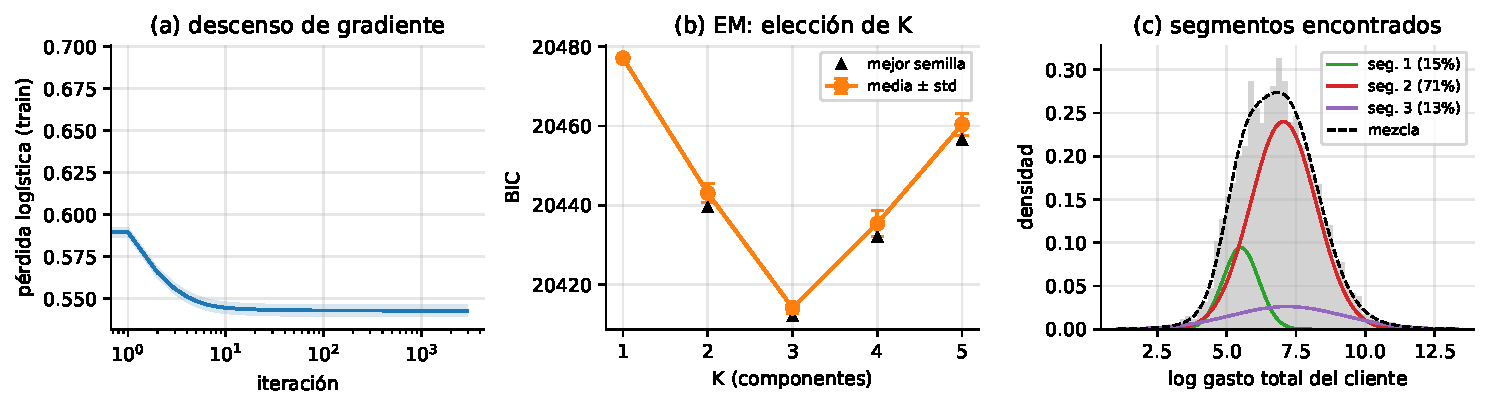
\includegraphics[width=\linewidth]{figuras/p1_logistica_em.pdf}
\caption{(a) Pérdida del descenso de gradiente (10 particiones). (b) BIC contra número de componentes. (c) Mezcla de 3 Gaussianas encontrada por EM sobre el log del gasto.}
\label{p2:fig:p1}
\end{figure}

\paragraph{Escalamiento.} Al pasar de 1\,000 a 5\,852 clientes (5\,256 en la logística, que solo usa clientes con historial antes del corte), el tiempo del descenso de gradiente sube de 0.12 a 0.41 s y el de EM de 0.04 a 0.29 s; la memoria pico, de 0.10 a 0.28 MB y de 0.15 a 0.71 MB (Figura~\ref{p2:fig:p1esc}). Ambos crecen de forma lineal con $n$, como se espera: cada iteración cuesta $O(nd)$ en la logística y $O(nK)$ en EM, y el número de iteraciones casi no cambia.

\begin{figure}[H]\centering
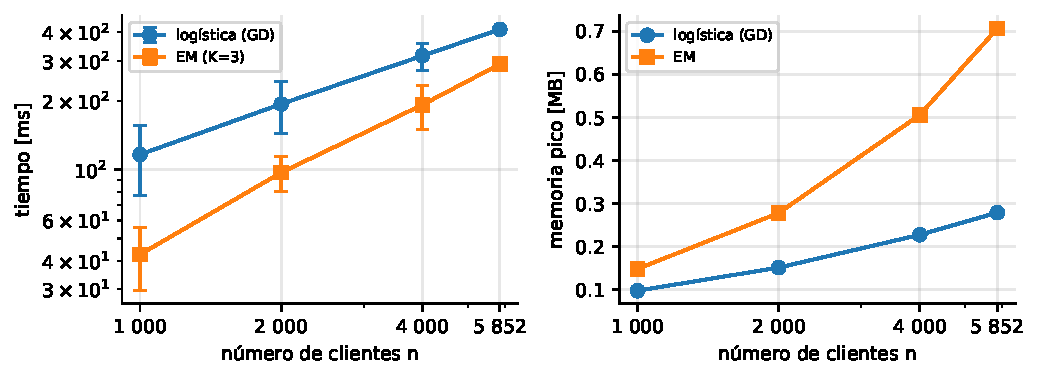
\includegraphics[width=0.8\linewidth]{figuras/p1_escalamiento.pdf}
\caption{Tiempo y memoria pico contra el número de clientes (10 submuestras por tamaño).}
\label{p2:fig:p1esc}
\end{figure}

% -----------------------------------------------------------------------------
\section*{2. Precios de productos relacionados (ingreso no convexo)}
\label{p2:sec:p2}

\paragraph{Modelo.} Se toman los 10 productos con más ventas. Sea $x_i\in[0.5,\,2.5]$ el precio del producto $i$ dividido entre su precio de referencia; la demanda del producto $i$ es
\[ D_i(\mathbf x)= q_i\,e^{-e\,(x_i-1)}\Big[(1-\lambda)+\lambda\,\sigma\big(k\,(c_i-x_i)\big)\Big]\prod_{j\in\text{cat}(i),\,j\ne i}\Big(\frac{x_j}{x_i}\Big)^{g}, \]
y el ingreso es $R(\mathbf x)=\sum_i \text{precio de referencia}_i\, x_i\, D_i(\mathbf x)$. Cada término viene de los datos o de la parte 1:
\begin{itemize}[itemsep=1pt]
  \item $q_i$ es la demanda media del producto y $c_i$ el precio del competidor (\texttt{comp\_1}) relativo al propio.
  \item $\lambda=0.153$ es la fracción de clientes que comparan precios: el peso del segmento de bajo gasto que encontró EM. Si el precio pasa al del competidor, esos clientes se van (la sigmoide $\sigma$).
  \item El último factor relaciona productos de la misma categoría: si uno sube de precio, parte de su demanda pasa a los otros.
  \item Se usaron $e=0.6$, $k=12$ y $g=0.3$.
\end{itemize}

\paragraph{Por qué no es convexo.} Para cada producto hay dos estrategias buenas: quedarse justo debajo del competidor para atraer a los que comparan, o subir mucho el precio y venderle solo a los leales. La Figura~\ref{p2:fig:corte} muestra el ingreso al mover el precio de un solo producto: tiene dos máximos. Con 10 productos las combinaciones se multiplican; al hacer ascenso de gradiente desde 100 puntos al azar se encontraron \textbf{16 óptimos locales distintos}, con ingresos entre 26\,810 y 27\,358.

\begin{figure}[H]\centering
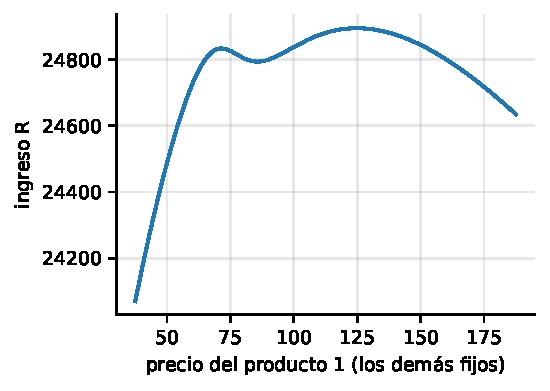
\includegraphics[width=0.42\linewidth]{figuras/p2_corte.pdf}
\caption{Ingreso al variar el precio del producto 1 con los demás fijos: dos máximos locales.}
\label{p2:fig:corte}
\end{figure}

\paragraph{Métodos.} Todos tienen el mismo presupuesto de $300d$ evaluaciones de $R$ (3\,000 para $d=10$):
\begin{itemize}[itemsep=1pt]
  \item \textbf{Gradiente con reinicios}: gradiente por diferencias centrales (cuesta $2d$ evaluaciones), paso de 0.05 en la dirección del gradiente; cuando deja de mejorar, reinicia en un punto al azar.
  \item \textbf{Hill Climbing}: cambia una coordenada con ruido Gaussiano ($\sigma=0.1$) y acepta solo si mejora; reinicia tras 100 intentos sin mejora.
  \item \textbf{Recocido simulado}: como el anterior, pero acepta empeorar con probabilidad $e^{\Delta/T}$; $T$ baja geométricamente durante todo el presupuesto.
  \item \textbf{GA real}: 40 individuos, torneo de 3, cruce BLX-0.5, mutación Gaussiana con probabilidad $1/d$ por gen y elitismo de 2.
  \item \textbf{PSO}: 30 partículas, $w=0.72$, $c_1=c_2=1.49$.
\end{itemize}
Como no se conoce el óptimo global, la brecha se mide contra el mejor ingreso que encontró cualquier método en cualquier semilla.

\begin{table}[H]\centering\footnotesize\setlength{\tabcolsep}{4pt}
\begin{tabular}{lccccc}\toprule
 & \multicolumn{3}{c}{brecha contra el mejor [\%]} & \multicolumn{2}{c}{tiempo [ms]}\\\cmidrule(lr){2-4}\cmidrule(lr){5-6}
Método & $d=10$ & $d=20$ & $d=40$ & $d=10$ & $d=40$\\\midrule
Gradiente + reinicios & 1.00 $\pm$ 0.56 & 21.76 $\pm$ 3.44 & 54.23 $\pm$ 3.24 & 33 & 179 \\
Hill Climbing & 0.43 $\pm$ 0.31 & 0.47 $\pm$ 0.43 & 9.97 $\pm$ 3.52 & 40 & 211 \\
Recocido simulado & 0.55 $\pm$ 0.59 & 0.22 $\pm$ 0.34 & 15.84 $\pm$ 14.07 & 40 & 216 \\
GA real & 0.03 $\pm$ 0.08 & 0.55 $\pm$ 0.37 & 2.15 $\pm$ 2.29 & 92 & 421 \\
PSO & 0.35 $\pm$ 0.40 & 6.16 $\pm$ 3.34 & 20.89 $\pm$ 7.85 & 32 & 180 \\
GA memético (extra) & 0.11 $\pm$ 0.23 & 0.31 $\pm$ 0.32 & 2.67 $\pm$ 2.53 & 75 & 279 \\\bottomrule
\end{tabular}
\caption{Precios: brecha contra el mejor valor encontrado (10 semillas, presupuesto $300d$). Memoria pico: 0.05 MB con $d=10$ y 0.2 MB con $d=40$ en todos los métodos.}
\label{p2:tab:precios}
\end{table}

\paragraph{Resultados.} Con $d=10$ todos los métodos quedan a menos de 1\,\% del mejor; el GA es el más consistente (0.03\,\%). El mejor ingreso encontrado (27\,358) es 10\,\% mayor que el de los precios actuales (24\,826). Al aumentar $d$ las diferencias crecen mucho (Tabla~\ref{p2:tab:precios} y Figura~\ref{p2:fig:p2}):
\begin{itemize}[itemsep=1pt]
  \item El gradiente con reinicios es el peor (54\,\% de brecha con $d=40$): cada gradiente gasta $2d$ evaluaciones, así que con el mismo presupuesto da pocos pasos y queda atrapado en el primer óptimo local.
  \item PSO converge rápido pero se estanca (21\,\% con $d=40$).
  \item Hill Climbing y Recocido Simulado van bien hasta $d=20$, pero con $d=40$ se quedan en 10--16\,\%.
  \item Los dos GA siguen cerca del mejor (2--3\,\%), porque la población explora varias zonas a la vez.
\end{itemize}
El GA es el más lento por el manejo de la población (0.4 s con $d=40$), pero todos son rápidos porque cada evaluación cuesta $O(d^2)$. La memoria crece de forma lineal con $d$ y es igual para todos.

\begin{figure}[H]\centering
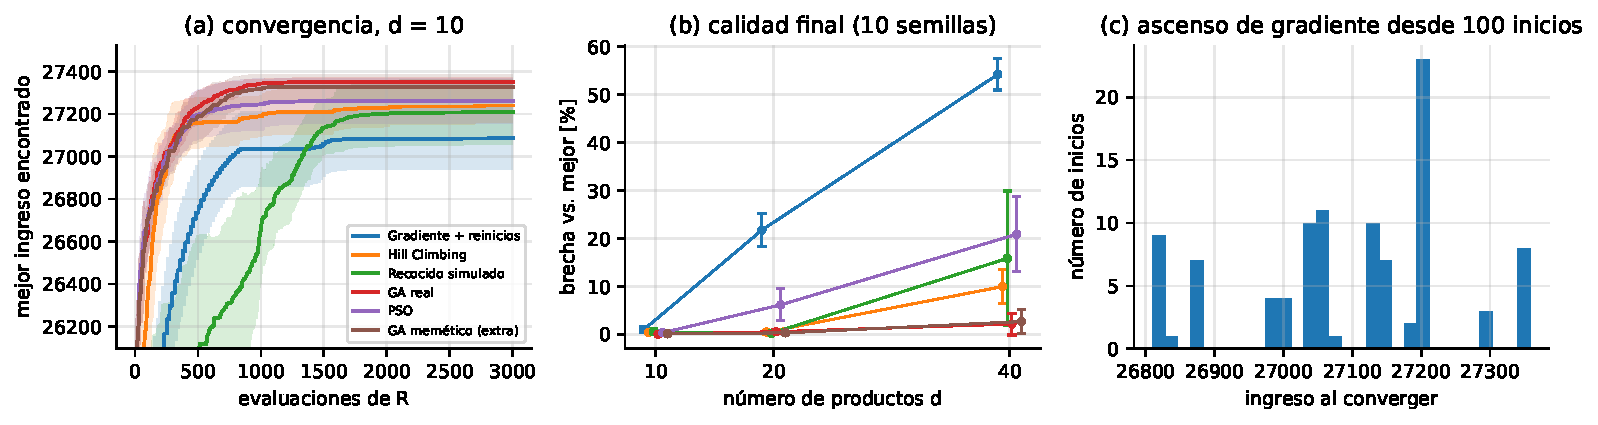
\includegraphics[width=\linewidth]{figuras/p2_precios.pdf}
\caption{(a) Mejor ingreso contra evaluaciones ($d=10$, media $\pm$ desviación). (b) Brecha final contra $d$. (c) Ingreso al que llega el ascenso de gradiente desde 100 inicios distintos.}
\label{p2:fig:p2}
\end{figure}

\begin{figure}[H]\centering
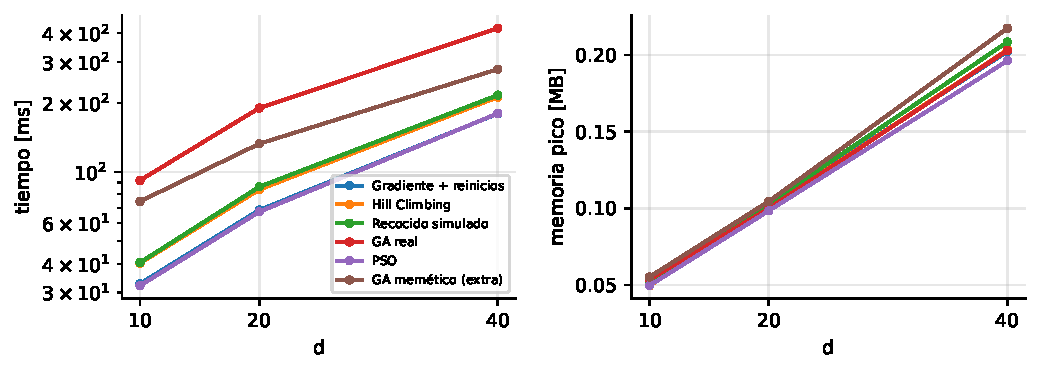
\includegraphics[width=0.8\linewidth]{figuras/p2_escalamiento.pdf}
\caption{Tiempo y memoria pico contra el número de productos.}
\label{p2:fig:p2esc}
\end{figure}

% -----------------------------------------------------------------------------
\section*{3. Guardias como juego de Stackelberg (Branch \& Bound y ACO)}
\label{p2:sec:p3}

\paragraph{Planteamiento.} La tienda (el líder) decide con qué probabilidad $p_z$ vigila cada zona y el ladrón (el seguidor) responde. Si roba en la zona $z$ gana $v_z$ y con probabilidad $p_z$ paga la multa $f$; si no roba se queda con lo que gana por la vía legal, $L$. Le conviene robar si $v_z-p_z f>L$, así que la zona queda disuadida si
\[ p_z\;\ge\;\frac{v_z-L}{f}=c_z. \]
Proteger la zona $z$ cuesta $c_z$ de presupuesto y evita perder $v_z$. Con presupuesto $\sum_z p_z\le B$, elegir qué zonas proteger es una mochila 0/1:
\[ \max\ \sum_z v_z y_z \quad\text{s.a.}\quad \sum_z c_z y_z\le B,\quad y_z\in\{0,1\}. \]

\paragraph{Caso del enunciado.} Con $v=(10,6,3)$, $f=20$, $L=1$ y $B=0.6$, los costos son $c=(0.45,\,0.25,\,0.10)$. Proteger las zonas 1 y 2 cuesta 0.70 (no cabe); proteger las zonas 1 y 3 cuesta 0.55 y vale $10+3=13$; las zonas 2 y 3 valen 9. El Branch \& Bound encuentra el óptimo de \textbf{13} (zonas 1 y 3, con $p_1=0.45$ y $p_3=0.10$) expandiendo 11 nodos, y ACO también llega a 13.

\begin{algorithm}[H]
\caption{Branch \& Bound para la mochila de guardias}
\label{p2:alg:bb}
\begin{algorithmic}[1]
\Require valores $v$, costos $c$, presupuesto $B$
\Ensure valor óptimo y zonas elegidas
\State ordenar zonas por $v_z/c_z$ de mayor a menor; mejor $\gets 0$
\State pila $\gets\{(i=0,\ \text{capacidad}=B,\ \text{valor}=0)\}$
\While{la pila no está vacía}
  \State sacar un nodo; actualizar mejor si su valor es mayor
  \If{$i=n$ \textbf{o} cota fraccionaria$(i,\text{capacidad},\text{valor})\le$ mejor} \textbf{podar} \EndIf
  \State meter ``sin la zona $i$'' (y sin sus copias idénticas)
  \If{$c_i\le$ capacidad} meter ``con la zona $i$'' (se explora primero) \EndIf
\EndWhile
\end{algorithmic}
\end{algorithm}

La cota es la mochila fraccionaria con las zonas que faltan (llenar en orden de $v/c$ y tomar una fracción de la última). Es una cota superior válida, así que podar con ella nunca elimina el óptimo; el código se verificó contra fuerza bruta en 300 instancias pequeñas (\texttt{code/pruebas.py}). La regla de copias idénticas evita explorar soluciones simétricas cuando varias zonas tienen el mismo valor. ACO usa 20 hormigas y 100 iteraciones: cada hormiga agrega zonas que todavía caben con probabilidad proporcional a $\tau^{1}\eta^{2}$, con $\eta=v/c$; la feromona se evapora ($\rho=0.1$) y se refuerza en la mejor solución.

\paragraph{De 30 a 120 zonas.} El valor de cada zona es el precio de un artículo de Online Retail II (en libras, la misma escala que $v=(10,6,3)$). Solo se usan artículos con $v>L$, porque los demás nunca conviene robarlos. El presupuesto es el 30\,\% del costo total y hay 10 instancias por tamaño.

\begin{table}[H]\centering\footnotesize\setlength{\tabcolsep}{4pt}
\begin{tabular}{rrrrrrr}\toprule
Zonas & Óptimo & Nodos B\&B (máx.) & B\&B [ms] & Brecha ACO [\%] & ACO exacto & ACO [ms]\\\midrule
30 & 34.17 & 209 (595) & 0.25 & 0.029 $\pm$ 0.090 & 90\% & 185 \\
60 & 67.39 & 280 (616) & 0.52 & 0.003 $\pm$ 0.009 & 90\% & 381 \\
90 & 102.85 & 654 (1435) & 1.47 & 0.015 $\pm$ 0.031 & 70\% & 574 \\
120 & 138.77 & 649 (1337) & 2.13 & 0.005 $\pm$ 0.011 & 80\% & 809 \\\bottomrule
\end{tabular}
\caption{Mochila de guardias: 10 instancias por tamaño. ``ACO exacto'' es el porcentaje de instancias donde ACO encontró el óptimo exacto. La memoria pico es menor a 0.04 MB en ambos métodos.}
\label{p2:tab:mochila}
\end{table}

El B\&B encontró y \emph{demostró} el óptimo en todas las instancias, con menos de 1\,500 nodos y en menos de 4 ms. ACO llega a menos de 0.03\,\% en promedio y encuentra el óptimo exacto en 70--90\,\% de las instancias, pero tarda entre 380 y 740 veces más y no puede garantizar que su solución sea la óptima (Figura~\ref{p2:fig:p3}). Aun así, el B\&B es exponencial en el peor caso: cuando valor y costo son casi proporcionales la cota fraccionaria poda poco. En estos datos no pasó porque la mayoría de los artículos son baratos y la razón $v/c=fv/(v-L)$ varía mucho entre zonas.

\begin{figure}[H]\centering
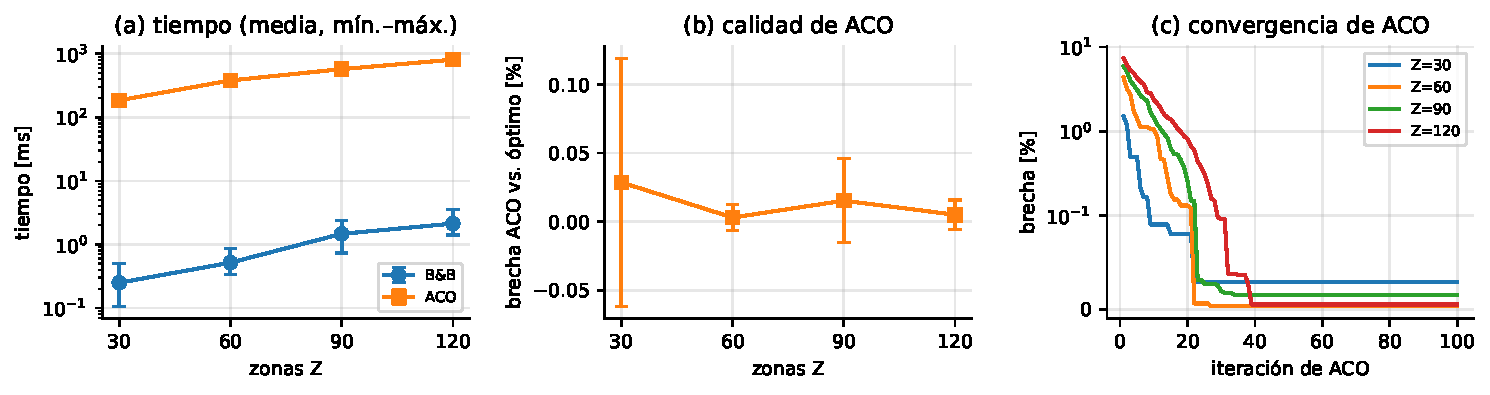
\includegraphics[width=\linewidth]{figuras/p3_mochila.pdf}
\caption{(a) Tiempo de B\&B y ACO. (b) Brecha de ACO contra el óptimo de B\&B. (c) Convergencia de ACO por iteración (promedio de 10 instancias).}
\label{p2:fig:p3}
\end{figure}

% -----------------------------------------------------------------------------
\section*{4. Guardia contra ladrón: minimax, alfa-beta y MCTS}
\label{p2:sec:p4}

\paragraph{Juego.} La tienda es una cuadrícula $n\times n$ con la salida en una esquina y tres zonas con artículos de valor 10, 6 y 3. El ladrón y el guardia se mueven por turnos una casilla (o se quedan). Si el ladrón pisa una zona toma el artículo. Las reglas para terminar son:
\begin{itemize}[itemsep=1pt]
  \item si el guardia llega a la casilla del ladrón, lo atrapa y la utilidad es $-20$ (la multa);
  \item si el ladrón llega a la salida con botín, escapa y la utilidad es el botín;
  \item si se acaban los turnos, la utilidad es 0.
\end{itemize}
Es un juego de suma cero: el ladrón maximiza y el guardia minimiza. Cuando la búsqueda se corta, una función de evaluación estima el valor con el botín (descontado por la distancia a la salida), la cercanía a los artículos que quedan y la cercanía al guardia.

\paragraph{Métodos.}
\begin{itemize}[itemsep=1pt]
  \item \textbf{Minimax} con profundidad limitada.
  \item \textbf{Alfa-beta} con dos órdenes de jugadas: aleatorio, o ``bueno'' (primero las jugadas con mejor evaluación para quien mueve).
  \item \textbf{MCTS con UCT}: 500 iteraciones de selección con $\bar u+1.4\sqrt{\ln N/n}$, expansión, simulación aleatoria hasta el final y retropropagación.
\end{itemize}

\begin{table}[H]\centering\small
\begin{tabular}{llrrr}\toprule
Cuadrícula & Profundidad & Minimax & Alfa-beta (aleatorio) & Alfa-beta (buen orden)\\\midrule
5$\times$5 & 2 & 17 & 13 & 10 \\
5$\times$5 & 4 & 289 & 130 & 70 \\
5$\times$5 & 6 & 4\,864 & 880 & 385 \\
5$\times$5 & 8 & -- & 5\,996 & 1\,771 \\
4$\times$4 & 8 & 63\,874 & 4\,668 & 1\,411 \\
6$\times$6 & 8 & -- & 7\,289 & 1\,395 \\\bottomrule
\end{tabular}
\caption{Nodos expandidos para decidir la primera jugada (promedio de 10 tableros). ``--'': no se corrió minimax a profundidad 8 en tableros grandes por ser demasiado lento.}
\label{p2:tab:nodos}
\end{table}

\paragraph{Resultados de la búsqueda.} En los 120 casos probados (100 con minimax, que no se corrió a profundidad 8 en $5\times5$ ni en $6\times6$), todas las variantes dieron exactamente el mismo valor en la raíz: la poda no cambia el resultado, solo evita trabajo. El ahorro crece con la profundidad (Tabla~\ref{p2:tab:nodos} y Figura~\ref{p2:fig:p4}):
\begin{itemize}[itemsep=1pt]
  \item a profundidad 6, alfa-beta con buen orden expande 12.6 veces menos nodos que minimax;
  \item en $4\times4$ a profundidad 8, el ahorro es de 45 veces (63\,874 contra 1\,411 nodos).
\end{itemize}
El factor de ramificación efectivo ($N^{1/d}$) a profundidad 6 en $5\times5$ es 4.1 con minimax, 3.1 con alfa-beta en orden aleatorio y 2.7 con buen orden, que se acerca al mínimo teórico de $\sqrt{4.1}\approx2.0$. El tamaño del tablero casi no influye, porque cada jugador tiene a lo más 5 movimientos sin importar $n$. La memoria de minimax y alfa-beta es mínima (0.001 MB, solo la pila de recursión); la de MCTS es mayor (0.23 MB) porque guarda el árbol.

\begin{figure}[H]\centering
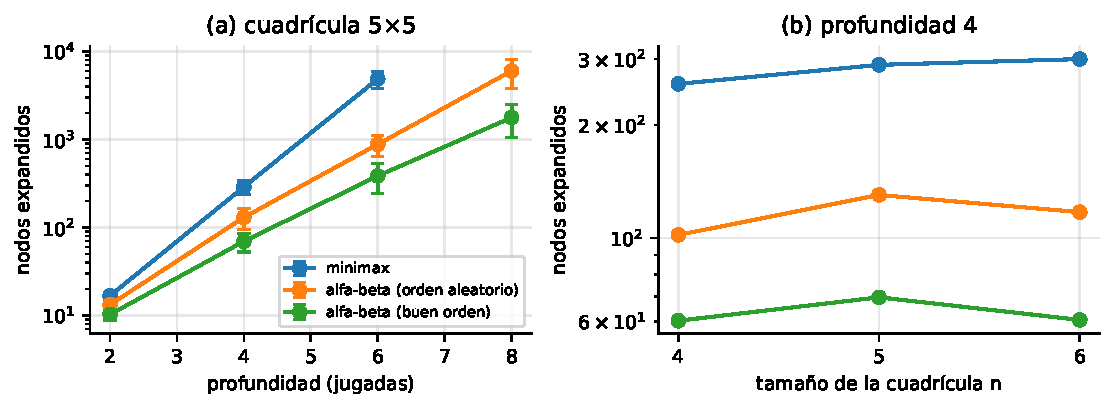
\includegraphics[width=0.8\linewidth]{figuras/p4_busqueda.pdf}
\caption{Nodos expandidos: (a) contra la profundidad en $5\times5$; (b) contra el tamaño del tablero a profundidad 4.}
\label{p2:fig:p4}
\end{figure}

\begin{table}[H]\centering\footnotesize\setlength{\tabcolsep}{4pt}
\begin{tabular}{llrrrrr}\toprule
Ladrón & Guardia & Utilidad ladrón & Escapa & Atrapado & $t$ ladrón [ms] & $t$ guardia [ms]\\\midrule
alfa-beta $p=4$ & alfa-beta $p=4$ & 0.9 $\pm$ 2.0 & 20\% & 0\% & 2 & 2 \\
alfa-beta $p=4$ & MCTS 500 & 2.2 $\pm$ 5.2 & 20\% & 0\% & 2 & 79 \\
MCTS 500 & alfa-beta $p=4$ & 0.3 $\pm$ 0.9 & 10\% & 0\% & 71 & 2 \\
MCTS 500 & MCTS 500 & 1.3 $\pm$ 3.2 & 20\% & 0\% & 73 & 70 \\
alfa-beta $p=4$ & aleatorio & 4.5 $\pm$ 6.6 & 40\% & 0\% & 2 & 0 \\\bottomrule
\end{tabular}
\caption{Partidas completas en $5\times5$ con 24 jugadas como máximo (10 tableros distintos). Los tiempos son el total de decisión por partida.}
\label{p2:tab:partidas}
\end{table}

\paragraph{Partidas.} El guardia con alfa-beta es el que menos deja ganar al ladrón, y uno que se mueve al azar deja escapar al 40\,\% de los ladrones (Tabla~\ref{p2:tab:partidas}). Nunca atrapan al ladrón, porque la multa de $-20$ hace que este prefiera irse sin nada antes que arriesgarse. MCTS juega de forma comparable a alfa-beta sin necesitar función de evaluación, pero tarda unas 35 veces más por partida porque cada iteración simula el juego hasta el final.

% -----------------------------------------------------------------------------
\section*{5. Clientes que aprenden: bandits, Q-learning y PPO}
\label{p2:sec:p5}

\paragraph{Bandits.} Un cliente frente a un artículo de valor $v=10$ con precio 9 tiene tres opciones, sin conocer $p$:
\begin{itemize}[itemsep=1pt]
  \item comprar: gana $v-\text{precio}=L=1$, más ruido $\mathcal N(0,1)$;
  \item robar: gana 10, o $10-20=-10$ si lo atrapan;
  \item irse: gana 0, más ruido.
\end{itemize}
Robar conviene si $10-20p>1$, es decir si $p<p^\star=(v-L)/f=0.45$, el mismo umbral de la parte 3. Se compararon tres estrategias en $2\times10^4$ visitas y 10 semillas:
\begin{itemize}[itemsep=1pt]
  \item $\varepsilon$-greedy con $\varepsilon=0.1$;
  \item UCB1, con las recompensas reescaladas a $[0,1]$;
  \item Thompson sampling con posterior Gaussiana ($\sigma=10$).
\end{itemize}

\begin{table}[H]\centering\footnotesize\setlength{\tabcolsep}{4pt}
\begin{tabular}{rlrrrrr}\toprule
$p$ & Algoritmo & Regret final & Robo (total) & Robo (últ. 1000) & Tiempo [ms] & Memoria [MB]\\\midrule
0.30 & Thompson & 610 $\pm$ 82 & 99.1\% & 99.9\% & 105 & 0.32 \\
0.30 & UCB1 & 4\,439 $\pm$ 212 & 93.4\% & 98.1\% & 81 & 0.31 \\
0.30 & $\varepsilon$-greedy & 5\,076 $\pm$ 654 & 92.7\% & 93.3\% & 38 & 0.31 \\
0.60 & Thompson & 911 $\pm$ 165 & 0.5\% & 0.1\% & 103 & 0.32 \\
0.60 & UCB1 & 5\,695 $\pm$ 474 & 4.0\% & 1.6\% & 83 & 0.31 \\
0.60 & $\varepsilon$-greedy & 2\,755 $\pm$ 110 & 3.4\% & 3.3\% & 40 & 0.31 \\\bottomrule
\end{tabular}
\caption{Bandits con $2\times10^4$ visitas y 10 semillas. Regret $=\sum_t(\mu^\star-\mu_{a_t})$.}
\label{p2:tab:bandits}
\end{table}

Los clientes aprenden lo correcto: con $p=0.30$ terminan robando casi siempre y con $p=0.60$ casi nunca (Tabla~\ref{p2:tab:bandits}). Thompson tiene el menor regret en ambos casos. $\varepsilon$-greedy tiene regret lineal, porque explora el 10\,\% del tiempo para siempre. UCB1 explora mucho al principio, porque las recompensas van de $-10$ a 10 y sus intervalos de confianza son anchos; aun así su regret crece de forma logarítmica. El barrido de $p$ (Figura~\ref{p2:fig:bandits}c) muestra que el cliente pasa de robar a no robar justo alrededor de $p^\star=0.45$: con $p=0.40$ roba el 69\,\% de las veces, con $p=0.45$ el 41\,\% y con $p=0.50$ el 17\,\%.

\begin{figure}[H]\centering
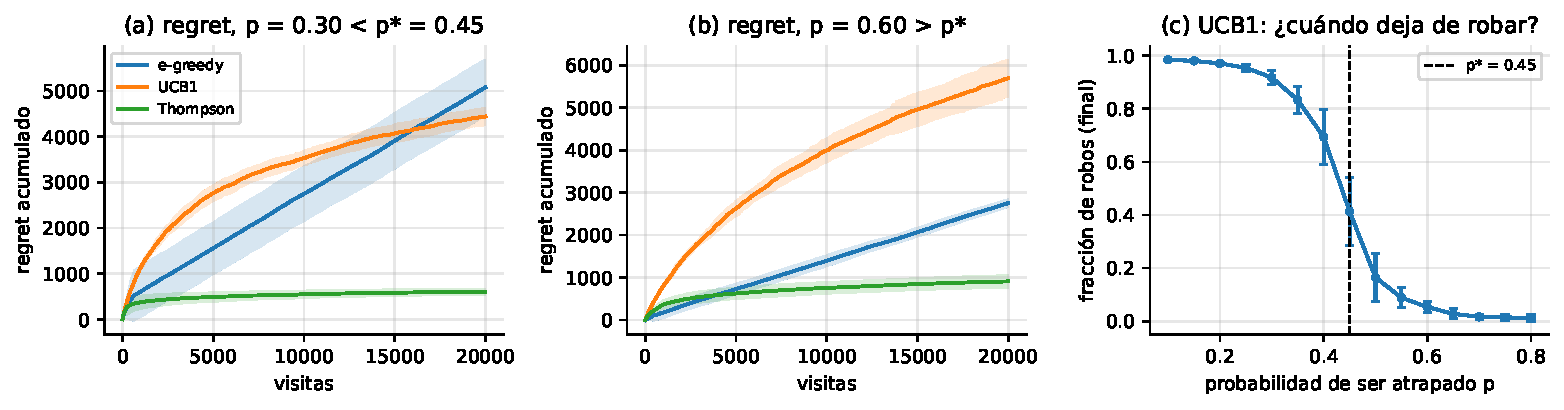
\includegraphics[width=\linewidth]{figuras/p5_bandits.pdf}
\caption{(a, b) Regret acumulado con $p$ debajo y encima de $p^\star$. (c) Fracción de robos al final contra $p$ (UCB1).}
\label{p2:fig:bandits}
\end{figure}

\paragraph{Q-learning con el guardia visible.} La tienda tiene tres zonas ($v=10,6,3$). El cliente ve en qué zona está el guardia al entrar ($g_0$), elige a qué zona ir y luego si compra, roba o se va. Mientras tanto el guardia se mueve a $g_1$ según la política de la tienda. Si roba en la zona donde quedó el guardia lo atrapan con probabilidad 0.9; en las demás, la cámara lo atrapa con probabilidad 0.05. El cliente aprende con Q-learning tabular: estado $g_0$ y luego $(g_0,\text{zona})$, $\varepsilon=0.1$, tasa $\alpha=\max(1/n,\,0.02)$.

Se probaron cuatro políticas fijas de la tienda. La política de Stackelberg usa la cobertura mínima que disuade todas las zonas, $0.9\,c_z+0.05\,(1-c_z)\ge(v_z-L)/f$, repartiendo el resto en proporción: $c=(0.62,\,0.31,\,0.08)$.

\paragraph{PPO para el guardia.} La tienda aprende su política con PPO de Stable-Baselines3 contra clientes que siguen aprendiendo con Q-learning:
\begin{itemize}[itemsep=1pt]
  \item \textbf{Observación:} zona actual del guardia y tasa reciente de robos por zona.
  \item \textbf{Acción:} a qué zona moverse.
  \item \textbf{Recompensa:} menos el valor robado.
  \item \textbf{Entrenamiento:} $2\times10^4$ visitas por semilla, con $\gamma=0$ (cada visita se paga sola), \texttt{n\_steps}=1000, \texttt{batch\_size}=200, 10 épocas, tasa de aprendizaje $10^{-3}$ y coeficiente de entropía 0.02.
\end{itemize}

\begin{table}[H]\centering\small
\begin{tabular}{lrrrr}\toprule
Política del guardia & Robo (todo) & Robo (últimas 2000) & Pérdida por visita & Tiempo [s]\\\midrule
fijo en zona 1 & 87.4 $\pm$ 0.8\% & 88.3 $\pm$ 0.8\% & 4.96 $\pm$ 0.06 & 0.08 \\
rotación 1$\to$2$\to$3 & 86.4 $\pm$ 1.7\% & 88.1 $\pm$ 0.5\% & 7.09 $\pm$ 0.26 & 0.08 \\
uniforme & 59.1 $\pm$ 15.7\% & 60.7 $\pm$ 20.9\% & 4.02 $\pm$ 1.41 & 0.09 \\
Stackelberg (mixta) & 4.9 $\pm$ 0.9\% & 3.4 $\pm$ 1.0\% & 0.11 $\pm$ 0.03 & 0.21 \\
PPO (aprendida) & 10.7 $\pm$ 2.9\% & 3.3 $\pm$ 0.3\% & 0.11 $\pm$ 0.02 & 2.88 \\\bottomrule
\end{tabular}
\caption{Clientes con Q-learning contra distintas políticas del guardia ($2\times10^4$ visitas, 10 semillas).}
\label{p2:tab:guardia}
\end{table}

\paragraph{Resultados.} Las políticas predecibles fallan: si el guardia siempre está en la misma zona o rota en orden fijo, el cliente aprende dónde va a estar y roba en otra zona el 88\,\% de las veces. La uniforme no alcanza, porque la zona 1 necesita al menos 0.47 de cobertura y solo recibe $1/3$. La mezcla de Stackelberg baja el robo a 3.4\,\%. PPO, sin conocer el modelo, llega al mismo nivel (3.3\,$\pm$\,0.3\,\% al final, en las 10 semillas). La cobertura promedio que aprendió, $(0.52,\,0.30,\,0.18)$, cumple los tres umbrales: las probabilidades de atrapar son 0.49, 0.30 y 0.20, contra los mínimos de 0.45, 0.25 y 0.10. El piso de $\approx$3\,\% no se puede bajar con vigilancia: es la exploración de los clientes ($\varepsilon/3\approx0.033$ de robos al azar). El costo de aprender es que durante el entrenamiento el robo promedio es 10.7\,\%, y que PPO tarda 2.9 s por semilla contra 0.2 s de la política calculada; además necesita PyTorch, y la memoria máxima del proceso llegó a 750 MB (esta cifra incluye los datos cargados en las partes anteriores).

\begin{figure}[H]\centering
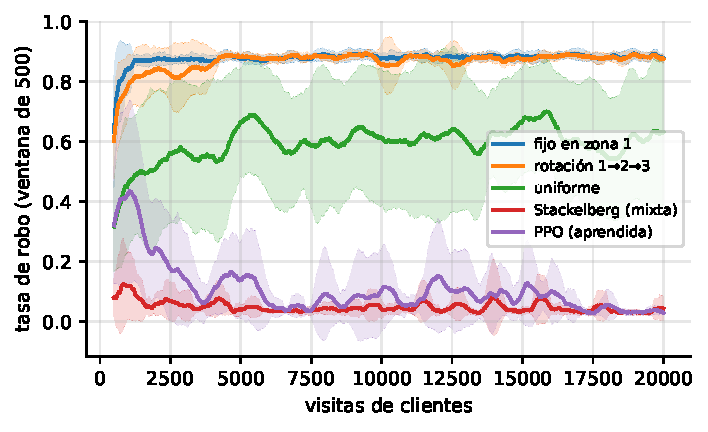
\includegraphics[width=0.72\linewidth]{figuras/p5_guardia.pdf}
\caption{Tasa de robo (ventana de 500 visitas) según la política del guardia; media $\pm$ desviación de 10 semillas.}
\label{p2:fig:guardia}
\end{figure}

% -----------------------------------------------------------------------------
\section*{Discusión: qué fue convexo y cuándo planear o aprender}
\label{p2:sec:discusion}

\paragraph{Convexo y no convexo.}
\begin{itemize}[itemsep=1pt]
  \item \textbf{Convexos:} la pérdida logística (demostrado arriba), por eso el descenso de gradiente llega al mismo mínimo desde cualquier inicio; y la mochila fraccionaria, que es un problema lineal y sirve como cota en el B\&B.
  \item \textbf{No convexos:} la verosimilitud de EM (el resultado depende de la semilla), el ingreso de los productos (16 óptimos locales), la mochila 0/1 (es discreta), los juegos de búsqueda y el objetivo de PPO (una red neuronal contra un rival que cambia).
\end{itemize}
En lo convexo basta un método local; en lo no convexo hacen falta reinicios, poblaciones (GA, PSO, ACO) o búsqueda exacta con cotas.

\paragraph{Planear o aprender.} Conviene \emph{planear} con búsqueda exacta y cotas válidas cuando el modelo se conoce y el problema es chico:
\begin{itemize}[itemsep=1pt]
  \item el B\&B resolvió la mochila de guardias de forma exacta en milisegundos, mientras que ACO tardó cientos de veces más sin garantía;
  \item alfa-beta da la misma jugada que minimax (la óptima para la profundidad elegida) expandiendo muchos menos nodos y con poca memoria.
\end{itemize}
Conviene \emph{aprender} cuando no se conocen los parámetros ($p$, el comportamiento de los clientes) o cuando el rival se adapta. Los bandits encuentran el umbral $p^\star$ sin conocerlo, y PPO recuperó una estrategia equivalente a la de Stackelberg sin saber nada del modelo. A cambio, aprender necesitó miles de interacciones (con robos mientras aprendía), más tiempo y mucha más memoria que calcular la solución. En la práctica, la tienda debería planear con lo que sabe (la cobertura de Stackelberg) y usar el aprendizaje para ajustar cuando los datos reales no coinciden con el modelo.

% -----------------------------------------------------------------------------
\section*{Crédito extra}
\label{p2:sec:extra}

\paragraph{Modelo híbrido búsqueda--bioinspirado (GA memético).} Es el mismo GA real, pero en cada generación se aplica Hill Climbing ($2d$ pasos) al mejor individuo; las evaluaciones del Hill Climbing cuentan dentro del mismo presupuesto. Así, el GA explora y el Hill Climbing refina. Con $d=20$ fue el mejor de los métodos bioinspirados (0.31\,\% contra 0.55\,\% del GA), con $d=40$ quedó prácticamente empatado con el GA (2.7\,\% contra 2.2\,\%, dentro de la desviación estándar), y en los tres tamaños superó a Hill Climbing y a PSO; a Recocido Simulado lo superó con $d=10$ y $d=40$, aunque con $d=20$ Recocido quedó un poco mejor (0.22\,\% contra 0.31\,\%) (Tabla~\ref{p2:tab:precios}).

\paragraph{Tablero de visualización.} El programa genera \texttt{results/dashboard.html}, una página que se abre en el navegador con un panel por parte y las tablas resumen. También genera la Figura~\ref{p2:fig:dashboard}.

\begin{figure}[H]\centering
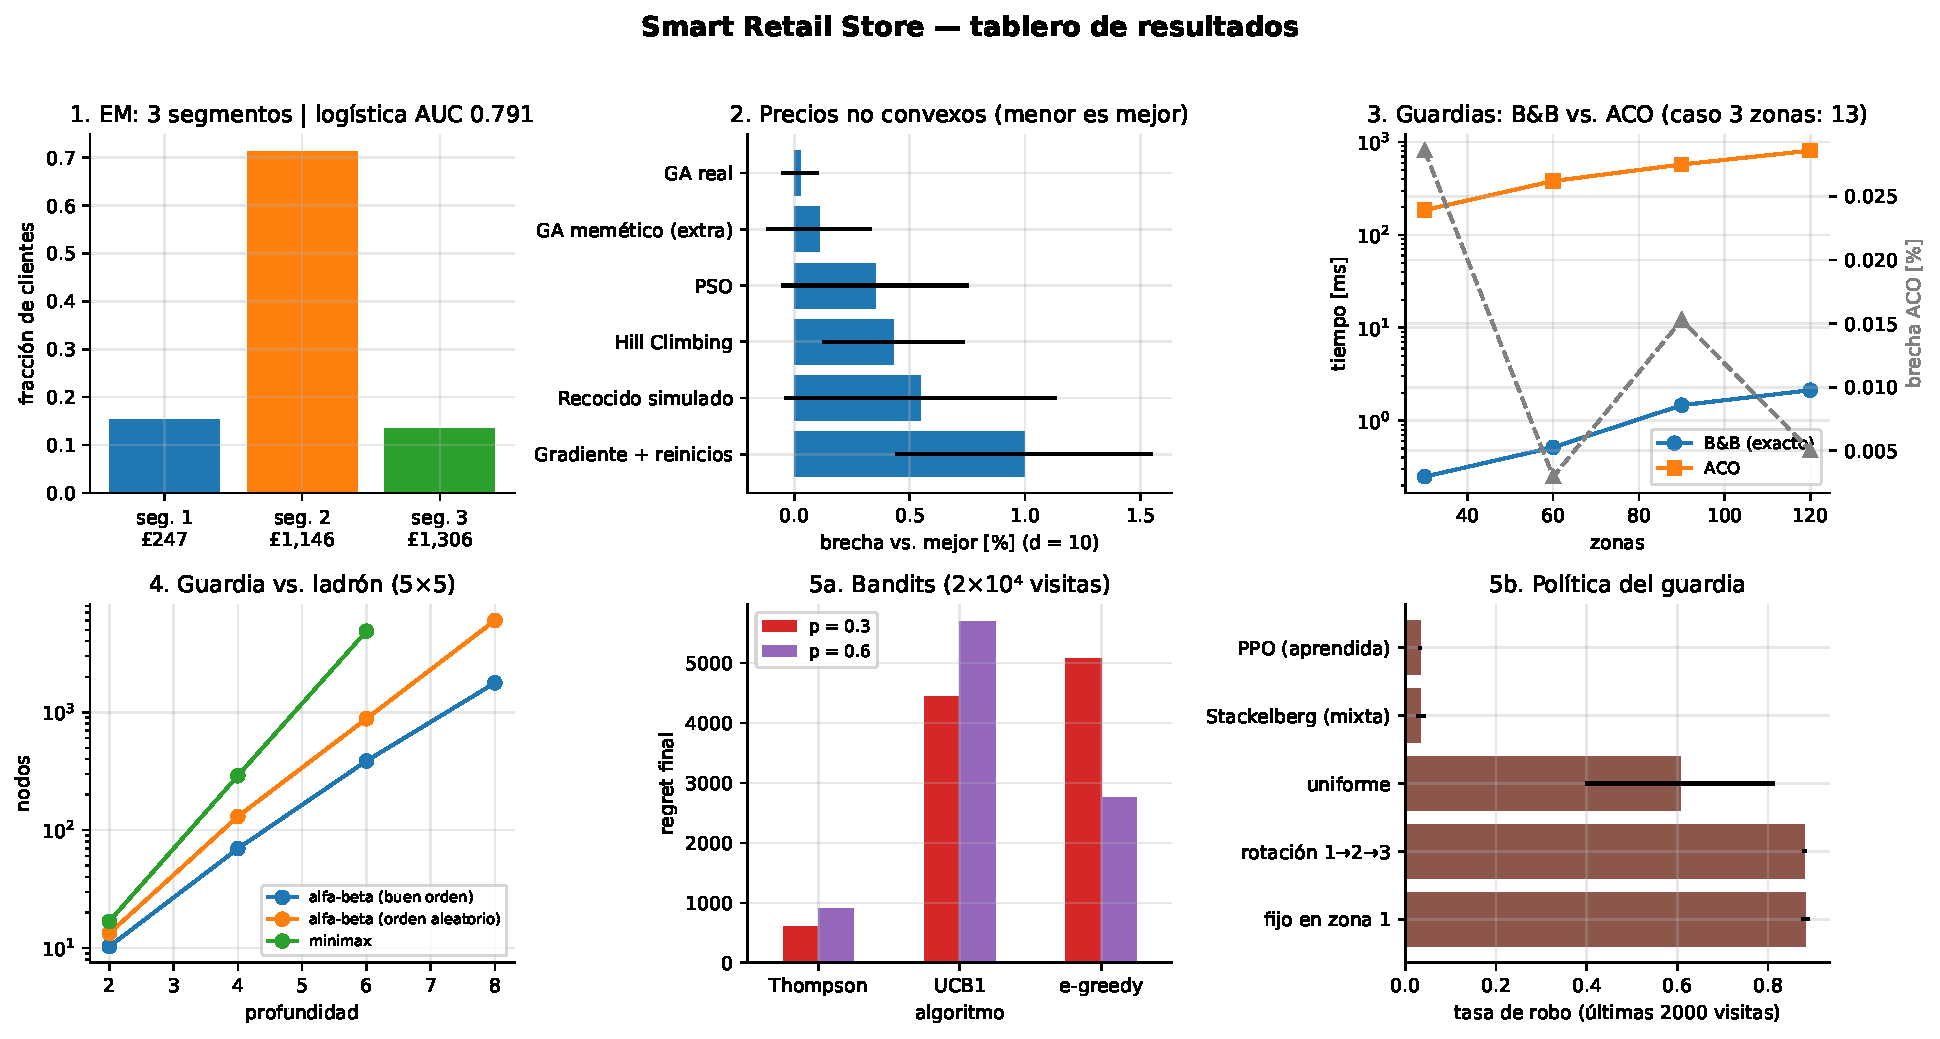
\includegraphics[width=\linewidth]{figuras/dashboard.pdf}
\caption{Tablero de resultados del Problema 2.}
\label{p2:fig:dashboard}
\end{figure}

\paragraph{Reproducir.} Las instrucciones para instalar las dependencias, descargar los datos y correr los experimentos están en el archivo \texttt{README.md} de la carpeta \texttt{problema2} del repositorio.

% -----------------------------------------------------------------------------
\section*{Referencias}
{\raggedright
\begin{enumerate}[label={[\arabic*]},leftmargin=*,itemsep=1pt]
\item S. Russell y P. Norvig. \emph{Artificial Intelligence: A Modern Approach}, 4.\textsuperscript{a} ed. Pearson, 2021.
\item A. P. Dempster, N. M. Laird y D. B. Rubin. Maximum likelihood from incomplete data via the EM algorithm. \emph{Journal of the Royal Statistical Society: Series B} 39(1):1--38, 1977.
\item S. Kirkpatrick, C. D. Gelatt y M. P. Vecchi. Optimization by simulated annealing. \emph{Science} 220(4598):671--680, 1983.
\item L. J. Eshelman y J. D. Schaffer. Real-coded genetic algorithms and interval-schemata. En \emph{Foundations of Genetic Algorithms 2}, pp.~187--202. Morgan Kaufmann, 1993.
\item J. Kennedy y R. Eberhart. Particle swarm optimization. En \emph{Proc. IEEE International Conference on Neural Networks}, pp.~1942--1948, 1995.
\item M. Tambe. \emph{Security and Game Theory: Algorithms, Deployed Systems, Lessons Learned}. Cambridge University Press, 2011.
\item M. Dorigo y T. Stützle. \emph{Ant Colony Optimization}. MIT Press, 2004.
\item D. E. Knuth y R. W. Moore. An analysis of alpha-beta pruning. \emph{Artificial Intelligence} 6(4):293--326, 1975.
\item L. Kocsis y C. Szepesvári. Bandit based Monte-Carlo planning. En \emph{Machine Learning: ECML 2006}, LNCS 4212, pp.~282--293. Springer, 2006.
\item P. Auer, N. Cesa-Bianchi y P. Fischer. Finite-time analysis of the multiarmed bandit problem. \emph{Machine Learning} 47:235--256, 2002.
\item W. R. Thompson. On the likelihood that one unknown probability exceeds another in view of the evidence of two samples. \emph{Biometrika} 25(3/4):285--294, 1933.
\item C. J. C. H. Watkins y P. Dayan. Q-learning. \emph{Machine Learning} 8:279--292, 1992.
\item J. Schulman, F. Wolski, P. Dhariwal, A. Radford y O. Klimov. Proximal policy optimization algorithms. arXiv:1707.06347, 2017.
\item A. Raffin, A. Hill, A. Gleave, A. Kanervisto, M. Ernestus y N. Dormann. Stable-Baselines3: reliable reinforcement learning implementations. \emph{Journal of Machine Learning Research} 22(268):1--8, 2021.
\item Online Retail II UCI (Kaggle). \url{https://www.kaggle.com/datasets/mashlyn/online-retail-ii-uci}, consultado el 9 de noviembre de 2026.
\item Retail Price Optimization (Kaggle). \url{https://www.kaggle.com/datasets/suddharshan/retail-price-optimization}, consultado el 9 de noviembre de 2026.
\end{enumerate}
\par}

\clearpage
\endgroup
 (desde reporte/P2_tienda.tex)
% Paquetes necesarios ademas de los del template: booktabs, float
% Las figuras se leen de figuras/ y las etiquetas usan el prefijo "p2:".
% =============================================================================

\begingroup
\renewcommand{\figurename}{Figura}
\renewcommand{\tablename}{Tabla}
\floatname{algorithm}{Algoritmo}
\algrenewcommand\algorithmicrequire{\textbf{Entrada:}}
\algrenewcommand\algorithmicensure{\textbf{Salida:}}
\algrenewcommand\algorithmicend{\textbf{fin}}
\algrenewcommand\algorithmicwhile{\textbf{mientras}}
\algrenewcommand\algorithmicdo{\textbf{hacer}}
\algrenewcommand\algorithmicif{\textbf{si}}
\algrenewcommand\algorithmicthen{\textbf{entonces}}
\algrenewcommand\algorithmicfor{\textbf{para}}
\algrenewcommand\algorithmicreturn{\textbf{devolver}}
\sloppy

% =============================================================================
\begin{abstract}
\noindent
Una tienda fija precios y coloca guardias, mientras que los clientes \emph{aprenden} si les conviene comprar, robar o irse sin conocer la probabilidad $p$ de ser atrapados (con una multa $f$ si los atrapan). Se ajustó un modelo logístico de compra con descenso de gradiente, demostrando que la pérdida es convexa, y se encontraron tres segmentos de clientes con EM; se optimizó el ingreso no convexo de $d=10$ productos relacionados con gradiente con reinicios, Hill Climbing, Recocido Simulado, un GA real y PSO con el mismo presupuesto de evaluaciones; se colocaron guardias como un juego de Stackelberg resuelto como mochila 0/1 con Branch \& Bound (óptimo de 13 en el caso del enunciado) y se comparó con ACO para 30--120 zonas; se jugó guardia contra ladrón con minimax, alfa-beta y MCTS; y se modeló a los clientes como bandits y como agentes de Q-learning, entrenando la política del guardia con PPO. Los experimentos usan datos de Kaggle (Online Retail II y Retail Price Optimization) y 10 semillas. El B\&B resolvió de forma exacta hasta 120 zonas en menos de 4 ms, el GA fue el método más robusto para los precios, y tanto la cobertura de Stackelberg como la política aprendida con PPO bajaron el robo a $\approx$3\,\%, contra 88\,\% con un guardia predecible.
\end{abstract}

% -----------------------------------------------------------------------------
\section*{Datos y configuración experimental}
\label{p2:sec:datos}

Se usaron dos de los datasets sugeridos, descargados de Kaggle el 9 de noviembre de 2026:
\begin{itemize}[itemsep=1pt]
  \item \textbf{Online Retail II UCI}:\newline \url{https://www.kaggle.com/datasets/mashlyn/online-retail-ii-uci}\newline Archivo \texttt{online\_retail\_II.csv}, con 1\,067\,371 renglones. Se quitaron las filas sin cliente, las facturas canceladas (las que empiezan con ``C''), las cantidades o precios $\le 0$ y los precios mayores al percentil 99.9. Quedaron 804\,774 transacciones de 5\,852 clientes. De aquí salen el modelo de compra, los segmentos de gasto y los valores de los artículos para el problema de los guardias.
  \item \textbf{Retail Price Optimization}:\newline \url{https://www.kaggle.com/datasets/suddharshan/retail-price-optimization}\newline Archivo \texttt{retail\_price.csv}, con 676 renglones. Se agrupó por producto: precio de referencia (mediana de \texttt{unit\_price}), demanda base (media de \texttt{qty}), precio del competidor (mediana de \texttt{comp\_1}) y categoría. De aquí sale el modelo de demanda para los precios.
\end{itemize}
El robo es simulado, con valores de artículos tomados de estos datos, como indica el enunciado.

\begin{table}[H]\centering\small
\begin{tabular}{lp{0.72\linewidth}}\toprule
Equipo & MacBook Pro, Apple M5 Pro, 24 GB de memoria, macOS 26.6.2 \\
Software & Python 3.13.15, NumPy 2.5.4, pandas 3.1.1, scikit-learn 1.9.1, PyTorch 2.15.0, Stable-Baselines3 2.9.2, Gymnasium 1.4.0 \\
Semillas & 10 semillas en todo lo estocástico; se reporta media $\pm$ desviación estándar \\
Tiempo & \texttt{time.perf\_counter} \\
Memoria & pico de \texttt{tracemalloc} en una corrida aparte con la semilla 0 (porque \texttt{tracemalloc} hace más lento el código); para PPO, memoria máxima del proceso \\
Tiempo total & 160 s para todo el problema (40, 43, 28, 5 y 45 s por parte) \\\bottomrule
\end{tabular}
\caption{Configuración de las pruebas.}
\label{p2:tab:setup}
\end{table}

% -----------------------------------------------------------------------------
\section*{1. Modelo de compra (regresión logística) y segmentos de clientes (EM)}
\label{p2:sec:p1}

\paragraph{Modelo de compra.} Para cada cliente se predice si vuelve a comprar en los últimos 90 días del periodo ($y=1$) a partir de su historial anterior a ese corte. Las variables son recencia, frecuencia (número de facturas), monto total, ticket promedio y antigüedad, con $\log(1+x)$ y estandarizadas. Quedaron 5\,256 clientes con historial antes del corte; el 43.6\,\% volvió a comprar.

La pérdida con regularización $\lambda=10^{-3}$ (sin regularizar el sesgo) es
\[ L(\mathbf w) = -\frac1n\sum_{i=1}^n\Big[y_i\log\sigma(\mathbf x_i^\top\mathbf w)+(1-y_i)\log\big(1-\sigma(\mathbf x_i^\top\mathbf w)\big)\Big] + \frac{\lambda}{2}\|\mathbf w_{1:}\|^2, \qquad \sigma(z)=\frac{1}{1+e^{-z}}, \]
y se minimiza con descenso de gradiente, $\mathbf w\gets\mathbf w-\eta\nabla L$, con $\eta=1$, hasta que $\|\nabla L\|<10^{-5}$.

\paragraph{La pérdida es convexa.} Usando $\sigma'(z)=\sigma(z)(1-\sigma(z))$, el gradiente y la Hessiana son
\[ \nabla L = \frac1n X^\top(\boldsymbol\sigma-\mathbf y)+\lambda\,\mathbf w_{1:}, \qquad
   \nabla^2 L = \frac1n X^\top S X + \lambda I', \quad S=\mathrm{diag}\big(\sigma_i(1-\sigma_i)\big), \]
donde $I'$ es la identidad con un cero en la posición del sesgo. Para cualquier vector $\mathbf z$,
\[ \mathbf z^\top\nabla^2 L\,\mathbf z = \frac1n\sum_{i=1}^n \sigma_i(1-\sigma_i)\,(\mathbf x_i^\top\mathbf z)^2 + \lambda\|\mathbf z_{1:}\|^2 \;\ge\; 0, \]
porque $0<\sigma_i<1$. La Hessiana es semidefinida positiva en todo punto, así que $L$ es convexa y cualquier mínimo local es global. Se comprobó también numéricamente: el menor eigenvalor de la Hessiana en la solución es $1.4\times10^{-3}>0$, y al arrancar desde 10 puntos al azar el descenso de gradiente llega siempre a la misma pérdida (0.543046 en los 10 casos, igual hasta la sexta cifra).

\paragraph{Resultados.} Con 10 particiones al azar 80/20, la exactitud en prueba es $0.725\pm0.011$ (adivinar siempre la clase mayoritaria da 0.564) y el AUC es $0.791\pm0.015$. El descenso de gradiente tarda unas 2\,500 iteraciones (0.34 s); son bastantes porque frecuencia, monto y ticket están muy correlacionados. Los pesos tienen el signo esperado: más frecuencia y más monto aumentan la probabilidad de volver, y más días sin comprar la reducen.

\paragraph{Segmentos con EM.} Se ajustó una mezcla de $K$ Gaussianas al logaritmo del gasto total de cada cliente con el algoritmo EM: el paso E calcula la probabilidad de que cada cliente pertenezca a cada componente y el paso M recalcula pesos, medias y varianzas. Se probó $K=1,\dots,5$ con 10 inicializaciones cada uno, y el BIC eligió $K=3$ (Figura~\ref{p2:fig:p1}b):
\begin{itemize}[itemsep=1pt]
  \item segmento 1 (15\,\%): gasto típico de \pounds247, clientes ocasionales;
  \item segmento 2 (71\,\%): gasto típico de \pounds1\,146, la mayoría de los clientes;
  \item segmento 3 (13\,\%): gasto típico de \pounds1\,306 pero con varianza muy grande, porque mezcla clientes pequeños con mayoristas.
\end{itemize}
A diferencia de la logística, EM no es convexo: con $K=3$ la log-verosimilitud final cambia con la semilla (entre $-10\,173.2$ y $-10\,171.3$), porque cada inicialización puede acabar en un máximo local distinto. Por eso se corre con varias semillas y se elige la mejor. El segmento 1 se usa en la parte 2 como los clientes que comparan precios.

\begin{figure}[H]\centering
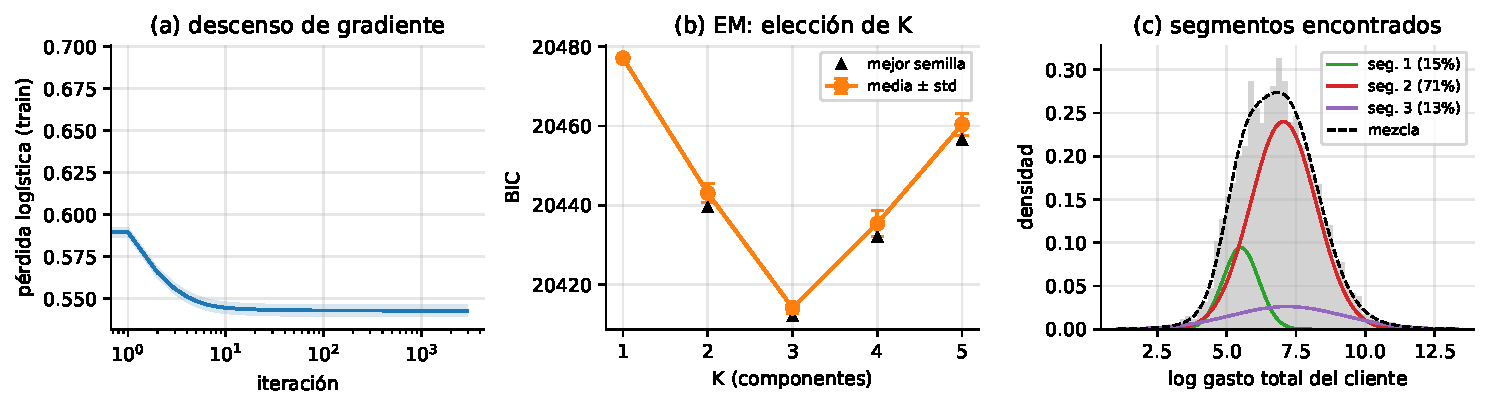
\includegraphics[width=\linewidth]{figuras/p1_logistica_em.pdf}
\caption{(a) Pérdida del descenso de gradiente (10 particiones). (b) BIC contra número de componentes. (c) Mezcla de 3 Gaussianas encontrada por EM sobre el log del gasto.}
\label{p2:fig:p1}
\end{figure}

\paragraph{Escalamiento.} Al pasar de 1\,000 a 5\,852 clientes (5\,256 en la logística, que solo usa clientes con historial antes del corte), el tiempo del descenso de gradiente sube de 0.12 a 0.41 s y el de EM de 0.04 a 0.29 s; la memoria pico, de 0.10 a 0.28 MB y de 0.15 a 0.71 MB (Figura~\ref{p2:fig:p1esc}). Ambos crecen de forma lineal con $n$, como se espera: cada iteración cuesta $O(nd)$ en la logística y $O(nK)$ en EM, y el número de iteraciones casi no cambia.

\begin{figure}[H]\centering
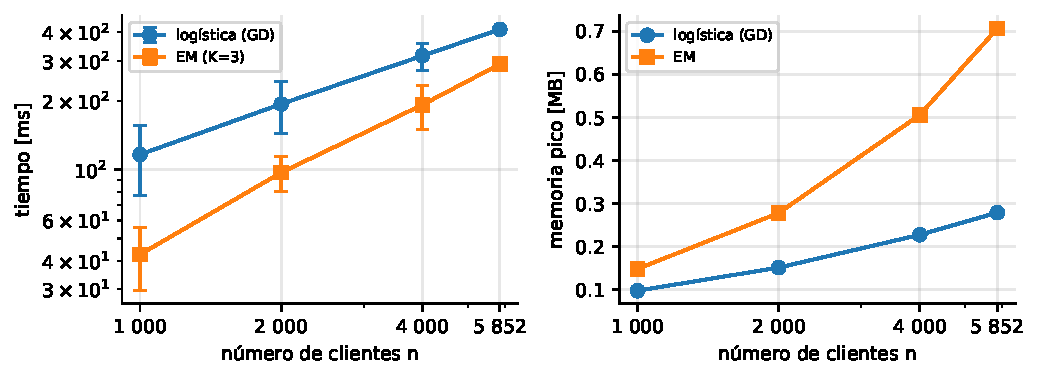
\includegraphics[width=0.8\linewidth]{figuras/p1_escalamiento.pdf}
\caption{Tiempo y memoria pico contra el número de clientes (10 submuestras por tamaño).}
\label{p2:fig:p1esc}
\end{figure}

% -----------------------------------------------------------------------------
\section*{2. Precios de productos relacionados (ingreso no convexo)}
\label{p2:sec:p2}

\paragraph{Modelo.} Se toman los 10 productos con más ventas. Sea $x_i\in[0.5,\,2.5]$ el precio del producto $i$ dividido entre su precio de referencia; la demanda del producto $i$ es
\[ D_i(\mathbf x)= q_i\,e^{-e\,(x_i-1)}\Big[(1-\lambda)+\lambda\,\sigma\big(k\,(c_i-x_i)\big)\Big]\prod_{j\in\text{cat}(i),\,j\ne i}\Big(\frac{x_j}{x_i}\Big)^{g}, \]
y el ingreso es $R(\mathbf x)=\sum_i \text{precio de referencia}_i\, x_i\, D_i(\mathbf x)$. Cada término viene de los datos o de la parte 1:
\begin{itemize}[itemsep=1pt]
  \item $q_i$ es la demanda media del producto y $c_i$ el precio del competidor (\texttt{comp\_1}) relativo al propio.
  \item $\lambda=0.153$ es la fracción de clientes que comparan precios: el peso del segmento de bajo gasto que encontró EM. Si el precio pasa al del competidor, esos clientes se van (la sigmoide $\sigma$).
  \item El último factor relaciona productos de la misma categoría: si uno sube de precio, parte de su demanda pasa a los otros.
  \item Se usaron $e=0.6$, $k=12$ y $g=0.3$.
\end{itemize}

\paragraph{Por qué no es convexo.} Para cada producto hay dos estrategias buenas: quedarse justo debajo del competidor para atraer a los que comparan, o subir mucho el precio y venderle solo a los leales. La Figura~\ref{p2:fig:corte} muestra el ingreso al mover el precio de un solo producto: tiene dos máximos. Con 10 productos las combinaciones se multiplican; al hacer ascenso de gradiente desde 100 puntos al azar se encontraron \textbf{16 óptimos locales distintos}, con ingresos entre 26\,810 y 27\,358.

\begin{figure}[H]\centering
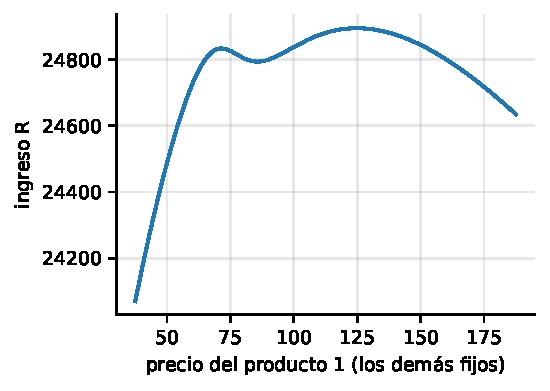
\includegraphics[width=0.42\linewidth]{figuras/p2_corte.pdf}
\caption{Ingreso al variar el precio del producto 1 con los demás fijos: dos máximos locales.}
\label{p2:fig:corte}
\end{figure}

\paragraph{Métodos.} Todos tienen el mismo presupuesto de $300d$ evaluaciones de $R$ (3\,000 para $d=10$):
\begin{itemize}[itemsep=1pt]
  \item \textbf{Gradiente con reinicios}: gradiente por diferencias centrales (cuesta $2d$ evaluaciones), paso de 0.05 en la dirección del gradiente; cuando deja de mejorar, reinicia en un punto al azar.
  \item \textbf{Hill Climbing}: cambia una coordenada con ruido Gaussiano ($\sigma=0.1$) y acepta solo si mejora; reinicia tras 100 intentos sin mejora.
  \item \textbf{Recocido simulado}: como el anterior, pero acepta empeorar con probabilidad $e^{\Delta/T}$; $T$ baja geométricamente durante todo el presupuesto.
  \item \textbf{GA real}: 40 individuos, torneo de 3, cruce BLX-0.5, mutación Gaussiana con probabilidad $1/d$ por gen y elitismo de 2.
  \item \textbf{PSO}: 30 partículas, $w=0.72$, $c_1=c_2=1.49$.
\end{itemize}
Como no se conoce el óptimo global, la brecha se mide contra el mejor ingreso que encontró cualquier método en cualquier semilla.

\begin{table}[H]\centering\footnotesize\setlength{\tabcolsep}{4pt}
\begin{tabular}{lccccc}\toprule
 & \multicolumn{3}{c}{brecha contra el mejor [\%]} & \multicolumn{2}{c}{tiempo [ms]}\\\cmidrule(lr){2-4}\cmidrule(lr){5-6}
Método & $d=10$ & $d=20$ & $d=40$ & $d=10$ & $d=40$\\\midrule
Gradiente + reinicios & 1.00 $\pm$ 0.56 & 21.76 $\pm$ 3.44 & 54.23 $\pm$ 3.24 & 33 & 179 \\
Hill Climbing & 0.43 $\pm$ 0.31 & 0.47 $\pm$ 0.43 & 9.97 $\pm$ 3.52 & 40 & 211 \\
Recocido simulado & 0.55 $\pm$ 0.59 & 0.22 $\pm$ 0.34 & 15.84 $\pm$ 14.07 & 40 & 216 \\
GA real & 0.03 $\pm$ 0.08 & 0.55 $\pm$ 0.37 & 2.15 $\pm$ 2.29 & 92 & 421 \\
PSO & 0.35 $\pm$ 0.40 & 6.16 $\pm$ 3.34 & 20.89 $\pm$ 7.85 & 32 & 180 \\
GA memético (extra) & 0.11 $\pm$ 0.23 & 0.31 $\pm$ 0.32 & 2.67 $\pm$ 2.53 & 75 & 279 \\\bottomrule
\end{tabular}
\caption{Precios: brecha contra el mejor valor encontrado (10 semillas, presupuesto $300d$). Memoria pico: 0.05 MB con $d=10$ y 0.2 MB con $d=40$ en todos los métodos.}
\label{p2:tab:precios}
\end{table}

\paragraph{Resultados.} Con $d=10$ todos los métodos quedan a menos de 1\,\% del mejor; el GA es el más consistente (0.03\,\%). El mejor ingreso encontrado (27\,358) es 10\,\% mayor que el de los precios actuales (24\,826). Al aumentar $d$ las diferencias crecen mucho (Tabla~\ref{p2:tab:precios} y Figura~\ref{p2:fig:p2}):
\begin{itemize}[itemsep=1pt]
  \item El gradiente con reinicios es el peor (54\,\% de brecha con $d=40$): cada gradiente gasta $2d$ evaluaciones, así que con el mismo presupuesto da pocos pasos y queda atrapado en el primer óptimo local.
  \item PSO converge rápido pero se estanca (21\,\% con $d=40$).
  \item Hill Climbing y Recocido Simulado van bien hasta $d=20$, pero con $d=40$ se quedan en 10--16\,\%.
  \item Los dos GA siguen cerca del mejor (2--3\,\%), porque la población explora varias zonas a la vez.
\end{itemize}
El GA es el más lento por el manejo de la población (0.4 s con $d=40$), pero todos son rápidos porque cada evaluación cuesta $O(d^2)$. La memoria crece de forma lineal con $d$ y es igual para todos.

\begin{figure}[H]\centering
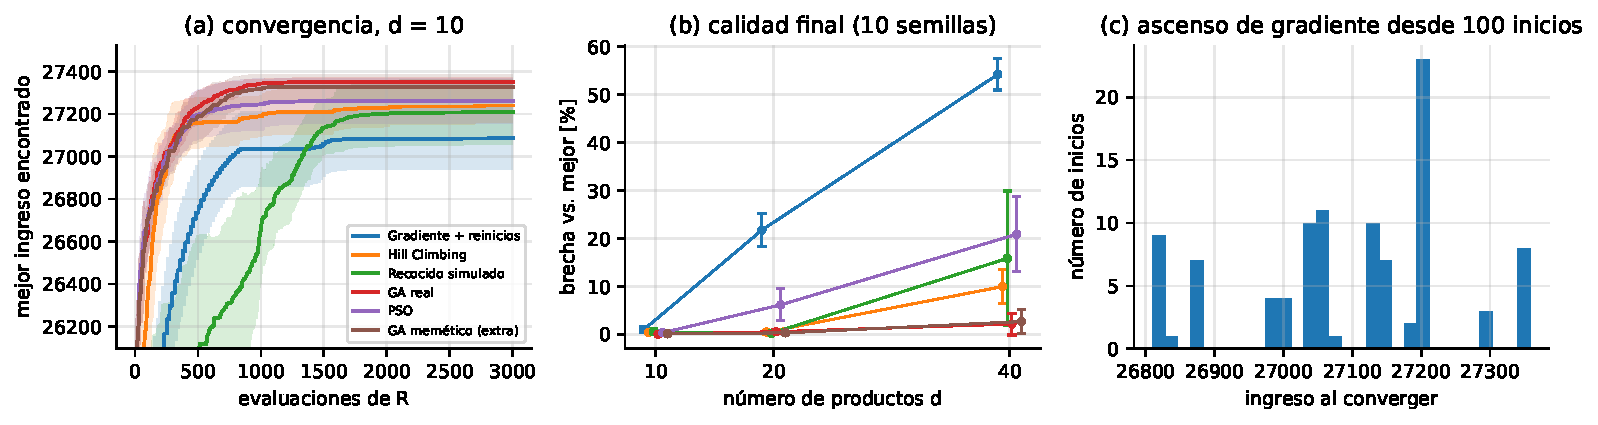
\includegraphics[width=\linewidth]{figuras/p2_precios.pdf}
\caption{(a) Mejor ingreso contra evaluaciones ($d=10$, media $\pm$ desviación). (b) Brecha final contra $d$. (c) Ingreso al que llega el ascenso de gradiente desde 100 inicios distintos.}
\label{p2:fig:p2}
\end{figure}

\begin{figure}[H]\centering
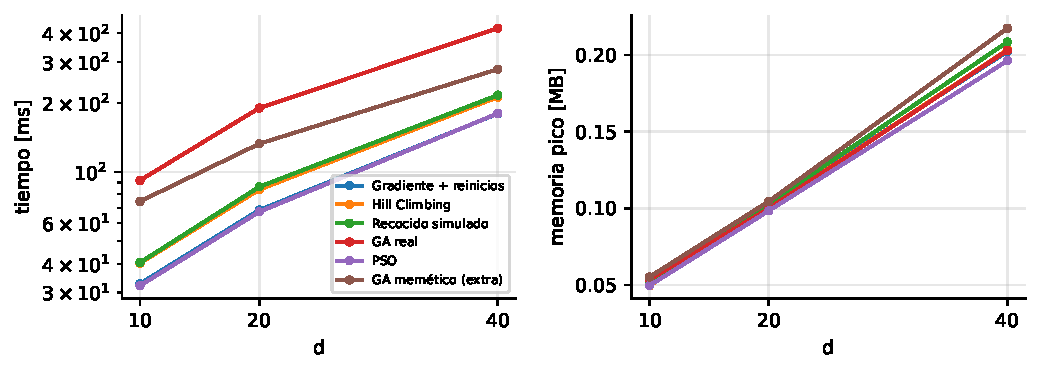
\includegraphics[width=0.8\linewidth]{figuras/p2_escalamiento.pdf}
\caption{Tiempo y memoria pico contra el número de productos.}
\label{p2:fig:p2esc}
\end{figure}

% -----------------------------------------------------------------------------
\section*{3. Guardias como juego de Stackelberg (Branch \& Bound y ACO)}
\label{p2:sec:p3}

\paragraph{Planteamiento.} La tienda (el líder) decide con qué probabilidad $p_z$ vigila cada zona y el ladrón (el seguidor) responde. Si roba en la zona $z$ gana $v_z$ y con probabilidad $p_z$ paga la multa $f$; si no roba se queda con lo que gana por la vía legal, $L$. Le conviene robar si $v_z-p_z f>L$, así que la zona queda disuadida si
\[ p_z\;\ge\;\frac{v_z-L}{f}=c_z. \]
Proteger la zona $z$ cuesta $c_z$ de presupuesto y evita perder $v_z$. Con presupuesto $\sum_z p_z\le B$, elegir qué zonas proteger es una mochila 0/1:
\[ \max\ \sum_z v_z y_z \quad\text{s.a.}\quad \sum_z c_z y_z\le B,\quad y_z\in\{0,1\}. \]

\paragraph{Caso del enunciado.} Con $v=(10,6,3)$, $f=20$, $L=1$ y $B=0.6$, los costos son $c=(0.45,\,0.25,\,0.10)$. Proteger las zonas 1 y 2 cuesta 0.70 (no cabe); proteger las zonas 1 y 3 cuesta 0.55 y vale $10+3=13$; las zonas 2 y 3 valen 9. El Branch \& Bound encuentra el óptimo de \textbf{13} (zonas 1 y 3, con $p_1=0.45$ y $p_3=0.10$) expandiendo 11 nodos, y ACO también llega a 13.

\begin{algorithm}[H]
\caption{Branch \& Bound para la mochila de guardias}
\label{p2:alg:bb}
\begin{algorithmic}[1]
\Require valores $v$, costos $c$, presupuesto $B$
\Ensure valor óptimo y zonas elegidas
\State ordenar zonas por $v_z/c_z$ de mayor a menor; mejor $\gets 0$
\State pila $\gets\{(i=0,\ \text{capacidad}=B,\ \text{valor}=0)\}$
\While{la pila no está vacía}
  \State sacar un nodo; actualizar mejor si su valor es mayor
  \If{$i=n$ \textbf{o} cota fraccionaria$(i,\text{capacidad},\text{valor})\le$ mejor} \textbf{podar} \EndIf
  \State meter ``sin la zona $i$'' (y sin sus copias idénticas)
  \If{$c_i\le$ capacidad} meter ``con la zona $i$'' (se explora primero) \EndIf
\EndWhile
\end{algorithmic}
\end{algorithm}

La cota es la mochila fraccionaria con las zonas que faltan (llenar en orden de $v/c$ y tomar una fracción de la última). Es una cota superior válida, así que podar con ella nunca elimina el óptimo; el código se verificó contra fuerza bruta en 300 instancias pequeñas (\texttt{code/pruebas.py}). La regla de copias idénticas evita explorar soluciones simétricas cuando varias zonas tienen el mismo valor. ACO usa 20 hormigas y 100 iteraciones: cada hormiga agrega zonas que todavía caben con probabilidad proporcional a $\tau^{1}\eta^{2}$, con $\eta=v/c$; la feromona se evapora ($\rho=0.1$) y se refuerza en la mejor solución.

\paragraph{De 30 a 120 zonas.} El valor de cada zona es el precio de un artículo de Online Retail II (en libras, la misma escala que $v=(10,6,3)$). Solo se usan artículos con $v>L$, porque los demás nunca conviene robarlos. El presupuesto es el 30\,\% del costo total y hay 10 instancias por tamaño.

\begin{table}[H]\centering\footnotesize\setlength{\tabcolsep}{4pt}
\begin{tabular}{rrrrrrr}\toprule
Zonas & Óptimo & Nodos B\&B (máx.) & B\&B [ms] & Brecha ACO [\%] & ACO exacto & ACO [ms]\\\midrule
30 & 34.17 & 209 (595) & 0.25 & 0.029 $\pm$ 0.090 & 90\% & 185 \\
60 & 67.39 & 280 (616) & 0.52 & 0.003 $\pm$ 0.009 & 90\% & 381 \\
90 & 102.85 & 654 (1435) & 1.47 & 0.015 $\pm$ 0.031 & 70\% & 574 \\
120 & 138.77 & 649 (1337) & 2.13 & 0.005 $\pm$ 0.011 & 80\% & 809 \\\bottomrule
\end{tabular}
\caption{Mochila de guardias: 10 instancias por tamaño. ``ACO exacto'' es el porcentaje de instancias donde ACO encontró el óptimo exacto. La memoria pico es menor a 0.04 MB en ambos métodos.}
\label{p2:tab:mochila}
\end{table}

El B\&B encontró y \emph{demostró} el óptimo en todas las instancias, con menos de 1\,500 nodos y en menos de 4 ms. ACO llega a menos de 0.03\,\% en promedio y encuentra el óptimo exacto en 70--90\,\% de las instancias, pero tarda entre 380 y 740 veces más y no puede garantizar que su solución sea la óptima (Figura~\ref{p2:fig:p3}). Aun así, el B\&B es exponencial en el peor caso: cuando valor y costo son casi proporcionales la cota fraccionaria poda poco. En estos datos no pasó porque la mayoría de los artículos son baratos y la razón $v/c=fv/(v-L)$ varía mucho entre zonas.

\begin{figure}[H]\centering
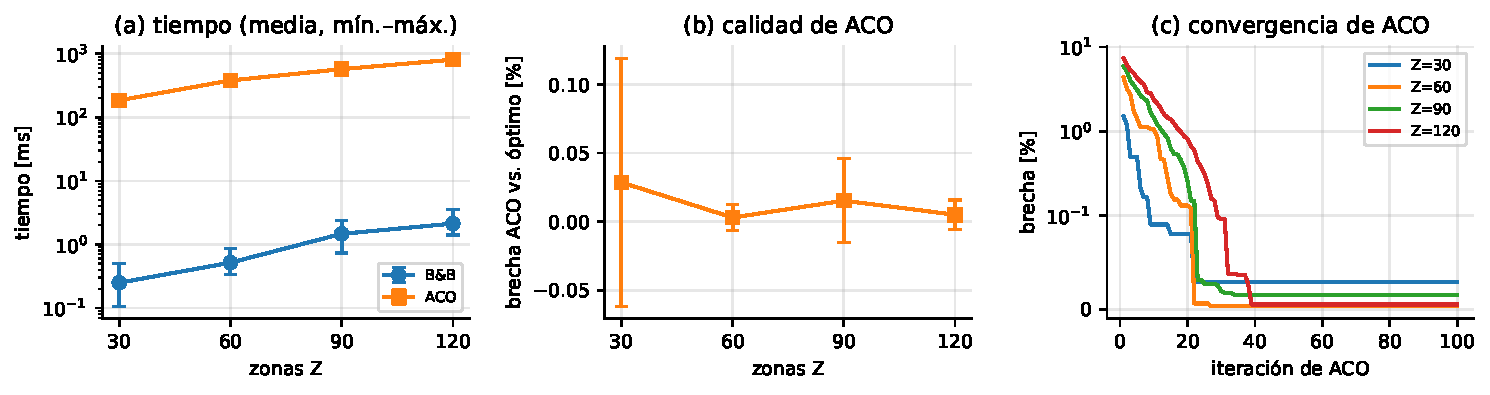
\includegraphics[width=\linewidth]{figuras/p3_mochila.pdf}
\caption{(a) Tiempo de B\&B y ACO. (b) Brecha de ACO contra el óptimo de B\&B. (c) Convergencia de ACO por iteración (promedio de 10 instancias).}
\label{p2:fig:p3}
\end{figure}

% -----------------------------------------------------------------------------
\section*{4. Guardia contra ladrón: minimax, alfa-beta y MCTS}
\label{p2:sec:p4}

\paragraph{Juego.} La tienda es una cuadrícula $n\times n$ con la salida en una esquina y tres zonas con artículos de valor 10, 6 y 3. El ladrón y el guardia se mueven por turnos una casilla (o se quedan). Si el ladrón pisa una zona toma el artículo. Las reglas para terminar son:
\begin{itemize}[itemsep=1pt]
  \item si el guardia llega a la casilla del ladrón, lo atrapa y la utilidad es $-20$ (la multa);
  \item si el ladrón llega a la salida con botín, escapa y la utilidad es el botín;
  \item si se acaban los turnos, la utilidad es 0.
\end{itemize}
Es un juego de suma cero: el ladrón maximiza y el guardia minimiza. Cuando la búsqueda se corta, una función de evaluación estima el valor con el botín (descontado por la distancia a la salida), la cercanía a los artículos que quedan y la cercanía al guardia.

\paragraph{Métodos.}
\begin{itemize}[itemsep=1pt]
  \item \textbf{Minimax} con profundidad limitada.
  \item \textbf{Alfa-beta} con dos órdenes de jugadas: aleatorio, o ``bueno'' (primero las jugadas con mejor evaluación para quien mueve).
  \item \textbf{MCTS con UCT}: 500 iteraciones de selección con $\bar u+1.4\sqrt{\ln N/n}$, expansión, simulación aleatoria hasta el final y retropropagación.
\end{itemize}

\begin{table}[H]\centering\small
\begin{tabular}{llrrr}\toprule
Cuadrícula & Profundidad & Minimax & Alfa-beta (aleatorio) & Alfa-beta (buen orden)\\\midrule
5$\times$5 & 2 & 17 & 13 & 10 \\
5$\times$5 & 4 & 289 & 130 & 70 \\
5$\times$5 & 6 & 4\,864 & 880 & 385 \\
5$\times$5 & 8 & -- & 5\,996 & 1\,771 \\
4$\times$4 & 8 & 63\,874 & 4\,668 & 1\,411 \\
6$\times$6 & 8 & -- & 7\,289 & 1\,395 \\\bottomrule
\end{tabular}
\caption{Nodos expandidos para decidir la primera jugada (promedio de 10 tableros). ``--'': no se corrió minimax a profundidad 8 en tableros grandes por ser demasiado lento.}
\label{p2:tab:nodos}
\end{table}

\paragraph{Resultados de la búsqueda.} En los 120 casos probados (100 con minimax, que no se corrió a profundidad 8 en $5\times5$ ni en $6\times6$), todas las variantes dieron exactamente el mismo valor en la raíz: la poda no cambia el resultado, solo evita trabajo. El ahorro crece con la profundidad (Tabla~\ref{p2:tab:nodos} y Figura~\ref{p2:fig:p4}):
\begin{itemize}[itemsep=1pt]
  \item a profundidad 6, alfa-beta con buen orden expande 12.6 veces menos nodos que minimax;
  \item en $4\times4$ a profundidad 8, el ahorro es de 45 veces (63\,874 contra 1\,411 nodos).
\end{itemize}
El factor de ramificación efectivo ($N^{1/d}$) a profundidad 6 en $5\times5$ es 4.1 con minimax, 3.1 con alfa-beta en orden aleatorio y 2.7 con buen orden, que se acerca al mínimo teórico de $\sqrt{4.1}\approx2.0$. El tamaño del tablero casi no influye, porque cada jugador tiene a lo más 5 movimientos sin importar $n$. La memoria de minimax y alfa-beta es mínima (0.001 MB, solo la pila de recursión); la de MCTS es mayor (0.23 MB) porque guarda el árbol.

\begin{figure}[H]\centering
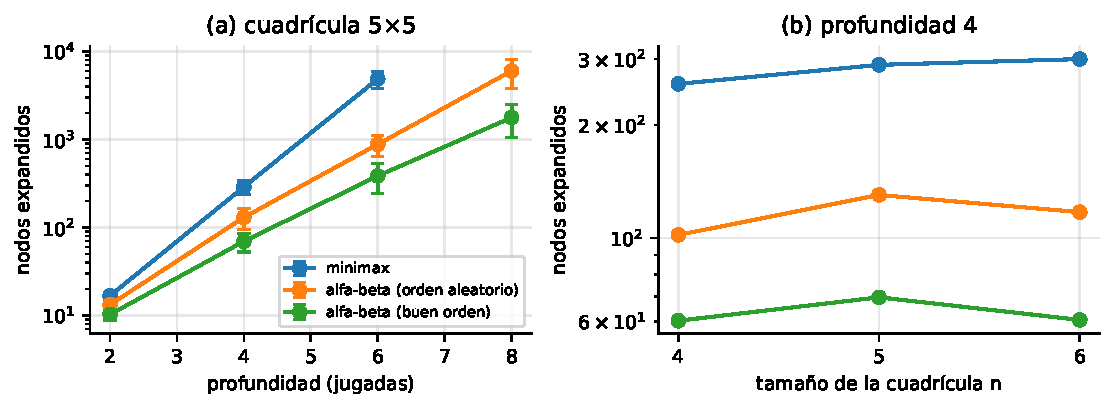
\includegraphics[width=0.8\linewidth]{figuras/p4_busqueda.pdf}
\caption{Nodos expandidos: (a) contra la profundidad en $5\times5$; (b) contra el tamaño del tablero a profundidad 4.}
\label{p2:fig:p4}
\end{figure}

\begin{table}[H]\centering\footnotesize\setlength{\tabcolsep}{4pt}
\begin{tabular}{llrrrrr}\toprule
Ladrón & Guardia & Utilidad ladrón & Escapa & Atrapado & $t$ ladrón [ms] & $t$ guardia [ms]\\\midrule
alfa-beta $p=4$ & alfa-beta $p=4$ & 0.9 $\pm$ 2.0 & 20\% & 0\% & 2 & 2 \\
alfa-beta $p=4$ & MCTS 500 & 2.2 $\pm$ 5.2 & 20\% & 0\% & 2 & 79 \\
MCTS 500 & alfa-beta $p=4$ & 0.3 $\pm$ 0.9 & 10\% & 0\% & 71 & 2 \\
MCTS 500 & MCTS 500 & 1.3 $\pm$ 3.2 & 20\% & 0\% & 73 & 70 \\
alfa-beta $p=4$ & aleatorio & 4.5 $\pm$ 6.6 & 40\% & 0\% & 2 & 0 \\\bottomrule
\end{tabular}
\caption{Partidas completas en $5\times5$ con 24 jugadas como máximo (10 tableros distintos). Los tiempos son el total de decisión por partida.}
\label{p2:tab:partidas}
\end{table}

\paragraph{Partidas.} El guardia con alfa-beta es el que menos deja ganar al ladrón, y uno que se mueve al azar deja escapar al 40\,\% de los ladrones (Tabla~\ref{p2:tab:partidas}). Nunca atrapan al ladrón, porque la multa de $-20$ hace que este prefiera irse sin nada antes que arriesgarse. MCTS juega de forma comparable a alfa-beta sin necesitar función de evaluación, pero tarda unas 35 veces más por partida porque cada iteración simula el juego hasta el final.

% -----------------------------------------------------------------------------
\section*{5. Clientes que aprenden: bandits, Q-learning y PPO}
\label{p2:sec:p5}

\paragraph{Bandits.} Un cliente frente a un artículo de valor $v=10$ con precio 9 tiene tres opciones, sin conocer $p$:
\begin{itemize}[itemsep=1pt]
  \item comprar: gana $v-\text{precio}=L=1$, más ruido $\mathcal N(0,1)$;
  \item robar: gana 10, o $10-20=-10$ si lo atrapan;
  \item irse: gana 0, más ruido.
\end{itemize}
Robar conviene si $10-20p>1$, es decir si $p<p^\star=(v-L)/f=0.45$, el mismo umbral de la parte 3. Se compararon tres estrategias en $2\times10^4$ visitas y 10 semillas:
\begin{itemize}[itemsep=1pt]
  \item $\varepsilon$-greedy con $\varepsilon=0.1$;
  \item UCB1, con las recompensas reescaladas a $[0,1]$;
  \item Thompson sampling con posterior Gaussiana ($\sigma=10$).
\end{itemize}

\begin{table}[H]\centering\footnotesize\setlength{\tabcolsep}{4pt}
\begin{tabular}{rlrrrrr}\toprule
$p$ & Algoritmo & Regret final & Robo (total) & Robo (últ. 1000) & Tiempo [ms] & Memoria [MB]\\\midrule
0.30 & Thompson & 610 $\pm$ 82 & 99.1\% & 99.9\% & 105 & 0.32 \\
0.30 & UCB1 & 4\,439 $\pm$ 212 & 93.4\% & 98.1\% & 81 & 0.31 \\
0.30 & $\varepsilon$-greedy & 5\,076 $\pm$ 654 & 92.7\% & 93.3\% & 38 & 0.31 \\
0.60 & Thompson & 911 $\pm$ 165 & 0.5\% & 0.1\% & 103 & 0.32 \\
0.60 & UCB1 & 5\,695 $\pm$ 474 & 4.0\% & 1.6\% & 83 & 0.31 \\
0.60 & $\varepsilon$-greedy & 2\,755 $\pm$ 110 & 3.4\% & 3.3\% & 40 & 0.31 \\\bottomrule
\end{tabular}
\caption{Bandits con $2\times10^4$ visitas y 10 semillas. Regret $=\sum_t(\mu^\star-\mu_{a_t})$.}
\label{p2:tab:bandits}
\end{table}

Los clientes aprenden lo correcto: con $p=0.30$ terminan robando casi siempre y con $p=0.60$ casi nunca (Tabla~\ref{p2:tab:bandits}). Thompson tiene el menor regret en ambos casos. $\varepsilon$-greedy tiene regret lineal, porque explora el 10\,\% del tiempo para siempre. UCB1 explora mucho al principio, porque las recompensas van de $-10$ a 10 y sus intervalos de confianza son anchos; aun así su regret crece de forma logarítmica. El barrido de $p$ (Figura~\ref{p2:fig:bandits}c) muestra que el cliente pasa de robar a no robar justo alrededor de $p^\star=0.45$: con $p=0.40$ roba el 69\,\% de las veces, con $p=0.45$ el 41\,\% y con $p=0.50$ el 17\,\%.

\begin{figure}[H]\centering
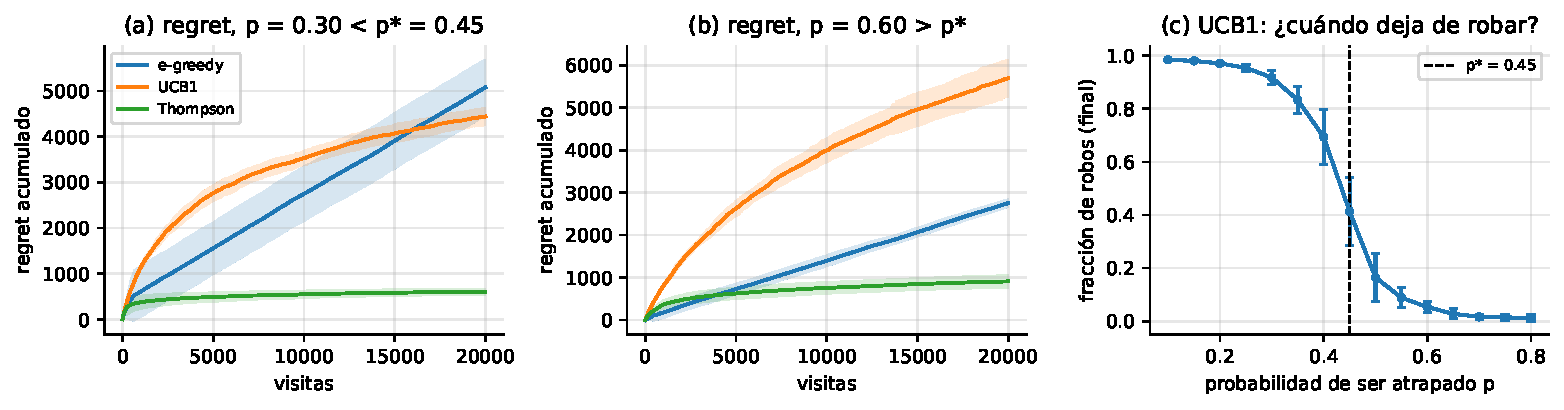
\includegraphics[width=\linewidth]{figuras/p5_bandits.pdf}
\caption{(a, b) Regret acumulado con $p$ debajo y encima de $p^\star$. (c) Fracción de robos al final contra $p$ (UCB1).}
\label{p2:fig:bandits}
\end{figure}

\paragraph{Q-learning con el guardia visible.} La tienda tiene tres zonas ($v=10,6,3$). El cliente ve en qué zona está el guardia al entrar ($g_0$), elige a qué zona ir y luego si compra, roba o se va. Mientras tanto el guardia se mueve a $g_1$ según la política de la tienda. Si roba en la zona donde quedó el guardia lo atrapan con probabilidad 0.9; en las demás, la cámara lo atrapa con probabilidad 0.05. El cliente aprende con Q-learning tabular: estado $g_0$ y luego $(g_0,\text{zona})$, $\varepsilon=0.1$, tasa $\alpha=\max(1/n,\,0.02)$.

Se probaron cuatro políticas fijas de la tienda. La política de Stackelberg usa la cobertura mínima que disuade todas las zonas, $0.9\,c_z+0.05\,(1-c_z)\ge(v_z-L)/f$, repartiendo el resto en proporción: $c=(0.62,\,0.31,\,0.08)$.

\paragraph{PPO para el guardia.} La tienda aprende su política con PPO de Stable-Baselines3 contra clientes que siguen aprendiendo con Q-learning:
\begin{itemize}[itemsep=1pt]
  \item \textbf{Observación:} zona actual del guardia y tasa reciente de robos por zona.
  \item \textbf{Acción:} a qué zona moverse.
  \item \textbf{Recompensa:} menos el valor robado.
  \item \textbf{Entrenamiento:} $2\times10^4$ visitas por semilla, con $\gamma=0$ (cada visita se paga sola), \texttt{n\_steps}=1000, \texttt{batch\_size}=200, 10 épocas, tasa de aprendizaje $10^{-3}$ y coeficiente de entropía 0.02.
\end{itemize}

\begin{table}[H]\centering\small
\begin{tabular}{lrrrr}\toprule
Política del guardia & Robo (todo) & Robo (últimas 2000) & Pérdida por visita & Tiempo [s]\\\midrule
fijo en zona 1 & 87.4 $\pm$ 0.8\% & 88.3 $\pm$ 0.8\% & 4.96 $\pm$ 0.06 & 0.08 \\
rotación 1$\to$2$\to$3 & 86.4 $\pm$ 1.7\% & 88.1 $\pm$ 0.5\% & 7.09 $\pm$ 0.26 & 0.08 \\
uniforme & 59.1 $\pm$ 15.7\% & 60.7 $\pm$ 20.9\% & 4.02 $\pm$ 1.41 & 0.09 \\
Stackelberg (mixta) & 4.9 $\pm$ 0.9\% & 3.4 $\pm$ 1.0\% & 0.11 $\pm$ 0.03 & 0.21 \\
PPO (aprendida) & 10.7 $\pm$ 2.9\% & 3.3 $\pm$ 0.3\% & 0.11 $\pm$ 0.02 & 2.88 \\\bottomrule
\end{tabular}
\caption{Clientes con Q-learning contra distintas políticas del guardia ($2\times10^4$ visitas, 10 semillas).}
\label{p2:tab:guardia}
\end{table}

\paragraph{Resultados.} Las políticas predecibles fallan: si el guardia siempre está en la misma zona o rota en orden fijo, el cliente aprende dónde va a estar y roba en otra zona el 88\,\% de las veces. La uniforme no alcanza, porque la zona 1 necesita al menos 0.47 de cobertura y solo recibe $1/3$. La mezcla de Stackelberg baja el robo a 3.4\,\%. PPO, sin conocer el modelo, llega al mismo nivel (3.3\,$\pm$\,0.3\,\% al final, en las 10 semillas). La cobertura promedio que aprendió, $(0.52,\,0.30,\,0.18)$, cumple los tres umbrales: las probabilidades de atrapar son 0.49, 0.30 y 0.20, contra los mínimos de 0.45, 0.25 y 0.10. El piso de $\approx$3\,\% no se puede bajar con vigilancia: es la exploración de los clientes ($\varepsilon/3\approx0.033$ de robos al azar). El costo de aprender es que durante el entrenamiento el robo promedio es 10.7\,\%, y que PPO tarda 2.9 s por semilla contra 0.2 s de la política calculada; además necesita PyTorch, y la memoria máxima del proceso llegó a 750 MB (esta cifra incluye los datos cargados en las partes anteriores).

\begin{figure}[H]\centering
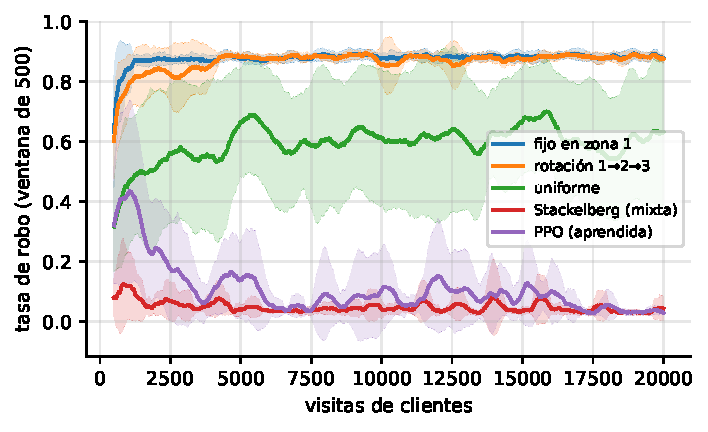
\includegraphics[width=0.72\linewidth]{figuras/p5_guardia.pdf}
\caption{Tasa de robo (ventana de 500 visitas) según la política del guardia; media $\pm$ desviación de 10 semillas.}
\label{p2:fig:guardia}
\end{figure}

% -----------------------------------------------------------------------------
\section*{Discusión: qué fue convexo y cuándo planear o aprender}
\label{p2:sec:discusion}

\paragraph{Convexo y no convexo.}
\begin{itemize}[itemsep=1pt]
  \item \textbf{Convexos:} la pérdida logística (demostrado arriba), por eso el descenso de gradiente llega al mismo mínimo desde cualquier inicio; y la mochila fraccionaria, que es un problema lineal y sirve como cota en el B\&B.
  \item \textbf{No convexos:} la verosimilitud de EM (el resultado depende de la semilla), el ingreso de los productos (16 óptimos locales), la mochila 0/1 (es discreta), los juegos de búsqueda y el objetivo de PPO (una red neuronal contra un rival que cambia).
\end{itemize}
En lo convexo basta un método local; en lo no convexo hacen falta reinicios, poblaciones (GA, PSO, ACO) o búsqueda exacta con cotas.

\paragraph{Planear o aprender.} Conviene \emph{planear} con búsqueda exacta y cotas válidas cuando el modelo se conoce y el problema es chico:
\begin{itemize}[itemsep=1pt]
  \item el B\&B resolvió la mochila de guardias de forma exacta en milisegundos, mientras que ACO tardó cientos de veces más sin garantía;
  \item alfa-beta da la misma jugada que minimax (la óptima para la profundidad elegida) expandiendo muchos menos nodos y con poca memoria.
\end{itemize}
Conviene \emph{aprender} cuando no se conocen los parámetros ($p$, el comportamiento de los clientes) o cuando el rival se adapta. Los bandits encuentran el umbral $p^\star$ sin conocerlo, y PPO recuperó una estrategia equivalente a la de Stackelberg sin saber nada del modelo. A cambio, aprender necesitó miles de interacciones (con robos mientras aprendía), más tiempo y mucha más memoria que calcular la solución. En la práctica, la tienda debería planear con lo que sabe (la cobertura de Stackelberg) y usar el aprendizaje para ajustar cuando los datos reales no coinciden con el modelo.

% -----------------------------------------------------------------------------
\section*{Crédito extra}
\label{p2:sec:extra}

\paragraph{Modelo híbrido búsqueda--bioinspirado (GA memético).} Es el mismo GA real, pero en cada generación se aplica Hill Climbing ($2d$ pasos) al mejor individuo; las evaluaciones del Hill Climbing cuentan dentro del mismo presupuesto. Así, el GA explora y el Hill Climbing refina. Con $d=20$ fue el mejor de los métodos bioinspirados (0.31\,\% contra 0.55\,\% del GA), con $d=40$ quedó prácticamente empatado con el GA (2.7\,\% contra 2.2\,\%, dentro de la desviación estándar), y en los tres tamaños superó a Hill Climbing y a PSO; a Recocido Simulado lo superó con $d=10$ y $d=40$, aunque con $d=20$ Recocido quedó un poco mejor (0.22\,\% contra 0.31\,\%) (Tabla~\ref{p2:tab:precios}).

\paragraph{Tablero de visualización.} El programa genera \texttt{results/dashboard.html}, una página que se abre en el navegador con un panel por parte y las tablas resumen. También genera la Figura~\ref{p2:fig:dashboard}.

\begin{figure}[H]\centering
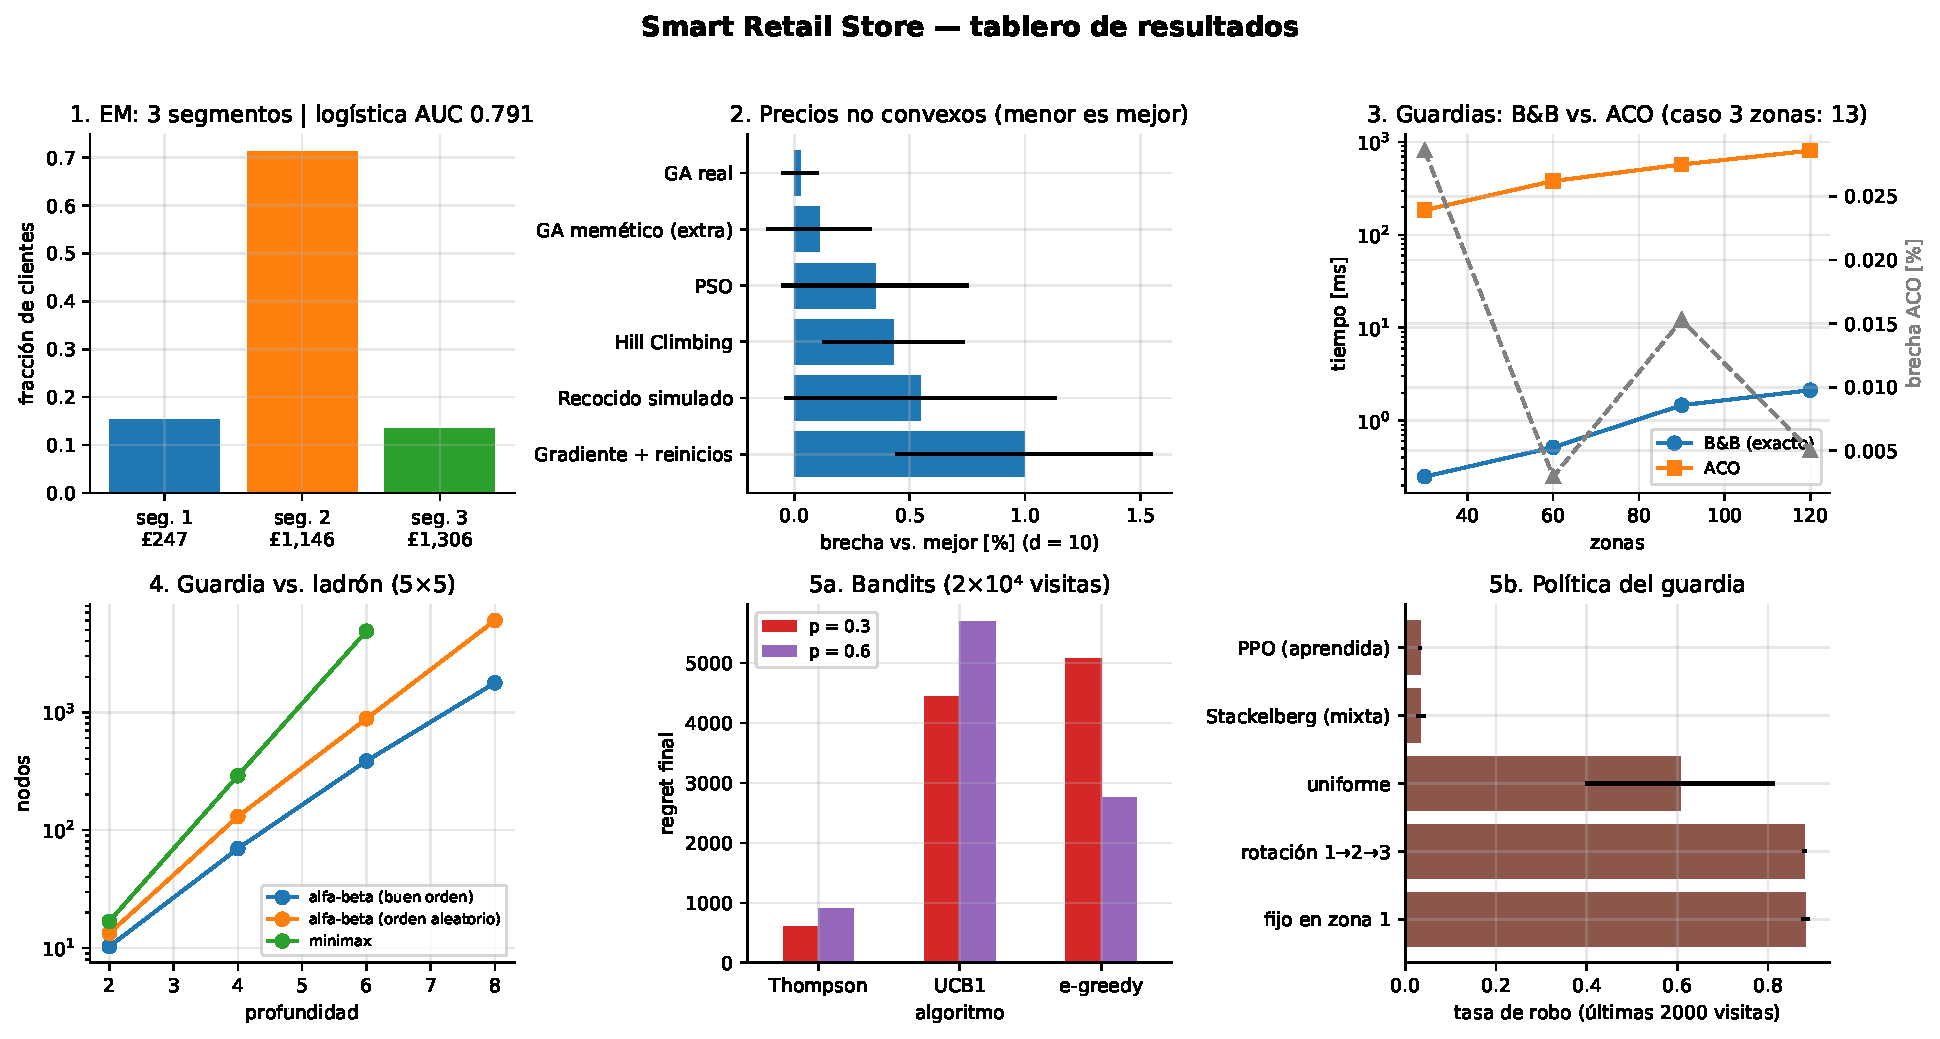
\includegraphics[width=\linewidth]{figuras/dashboard.pdf}
\caption{Tablero de resultados del Problema 2.}
\label{p2:fig:dashboard}
\end{figure}

\paragraph{Reproducir.} Las instrucciones para instalar las dependencias, descargar los datos y correr los experimentos están en el archivo \texttt{README.md} de la carpeta \texttt{problema2} del repositorio.

% -----------------------------------------------------------------------------
\section*{Referencias}
{\raggedright
\begin{enumerate}[label={[\arabic*]},leftmargin=*,itemsep=1pt]
\item S. Russell y P. Norvig. \emph{Artificial Intelligence: A Modern Approach}, 4.\textsuperscript{a} ed. Pearson, 2021.
\item A. P. Dempster, N. M. Laird y D. B. Rubin. Maximum likelihood from incomplete data via the EM algorithm. \emph{Journal of the Royal Statistical Society: Series B} 39(1):1--38, 1977.
\item S. Kirkpatrick, C. D. Gelatt y M. P. Vecchi. Optimization by simulated annealing. \emph{Science} 220(4598):671--680, 1983.
\item L. J. Eshelman y J. D. Schaffer. Real-coded genetic algorithms and interval-schemata. En \emph{Foundations of Genetic Algorithms 2}, pp.~187--202. Morgan Kaufmann, 1993.
\item J. Kennedy y R. Eberhart. Particle swarm optimization. En \emph{Proc. IEEE International Conference on Neural Networks}, pp.~1942--1948, 1995.
\item M. Tambe. \emph{Security and Game Theory: Algorithms, Deployed Systems, Lessons Learned}. Cambridge University Press, 2011.
\item M. Dorigo y T. Stützle. \emph{Ant Colony Optimization}. MIT Press, 2004.
\item D. E. Knuth y R. W. Moore. An analysis of alpha-beta pruning. \emph{Artificial Intelligence} 6(4):293--326, 1975.
\item L. Kocsis y C. Szepesvári. Bandit based Monte-Carlo planning. En \emph{Machine Learning: ECML 2006}, LNCS 4212, pp.~282--293. Springer, 2006.
\item P. Auer, N. Cesa-Bianchi y P. Fischer. Finite-time analysis of the multiarmed bandit problem. \emph{Machine Learning} 47:235--256, 2002.
\item W. R. Thompson. On the likelihood that one unknown probability exceeds another in view of the evidence of two samples. \emph{Biometrika} 25(3/4):285--294, 1933.
\item C. J. C. H. Watkins y P. Dayan. Q-learning. \emph{Machine Learning} 8:279--292, 1992.
\item J. Schulman, F. Wolski, P. Dhariwal, A. Radford y O. Klimov. Proximal policy optimization algorithms. arXiv:1707.06347, 2017.
\item A. Raffin, A. Hill, A. Gleave, A. Kanervisto, M. Ernestus y N. Dormann. Stable-Baselines3: reliable reinforcement learning implementations. \emph{Journal of Machine Learning Research} 22(268):1--8, 2021.
\item Online Retail II UCI (Kaggle). \url{https://www.kaggle.com/datasets/mashlyn/online-retail-ii-uci}, consultado el 9 de noviembre de 2026.
\item Retail Price Optimization (Kaggle). \url{https://www.kaggle.com/datasets/suddharshan/retail-price-optimization}, consultado el 9 de noviembre de 2026.
\end{enumerate}
\par}

\clearpage
\endgroup


\end{document}
